\documentclass{polytech/polytech}
\setlength\parindent{24pt}
\usepackage{lipsum}

\addbibresource{biblio.bib}

\schooldepartment{di}
\typereport{ppgldi4}
\reportyear{2018-2019}
\title{Rapport Projet Programmation et Génie Logiciel}
\subtitle{Développement d’un logiciel de contrôle de l’ordinateur par analyse des mouvements des yeux avec le dispositif Tobii}
\reportlogo{polytech/polytech}
           
\student{Yann}{Galan}{yann.galan@etu.univ-tours.fr}
\student{Vincent}{Rabier}{vincent.rabier@etu.univ-tours.fr}

\academicsupervisor[di]{Mohamed}{Slimane}{mohamed.slimane@univ-tours.fr}
\academicsupervisor[di]{Donatello}{Conte}{donatello.conte@univ-tours.fr}

\resume{
Le contrôle d'application par des dispositifs de contrôle tel que les souris est considéré de nos jours comme optimal. Cependant ce type de contrôleur n'est pas utilisable pour tout le monde. Ce projet consiste à développer une application pouvant être utilisée par le plus grand nombre. Elle met en relation le dispositif de suivi oculaire de la marque Tobii et une application du type jeu vidéo. Nous avons réalisé au cours de ce projet un jeu vidéo dont le point central était d'être utilisable uniquement en utilisant les yeux. Nous avons réalisé plusieurs mini-jeux ayant tous pour but de tester et d'améliorer un aspect des compétences des utilisateurs (ex: la mémoire, la rapidité, l'acuité visuelle). Ce projet a été réalisé dans le langage C++ en utilisant plusieurs bibliothèques visuelles. Nous avons également produit plusieurs documents de génie logiciel que vous pouvez consulter dans ce document.
}

\motcle{Tobii}
\motcle{suivi oculaire}
\motcle{C++}
\motcle{SDL}
\motcle{jeux vidéos}
             
\abstract{
Nowadays, we consider that application devices such as  mouse are optimal. However, this type of controller is not usable for everyone. This project consists in developing an application that can be used by as many people as possible. It connects the Tobii eye tracking device with a video game application. We realized a video game whose central point was to be used only by the eye tracking technology. We have made several mini-games, all aimed at testing and improving users' skills (eg memory, speed, visual acuity). This project was realized in C ++ using several visual libraries. We have also produced several software engineering documents that you can read in this document.
}
\keyword{eyetracking}
\keyword{Tobii}
\keyword{C++}
\keyword{SDL}
\keyword{video game}

\begin{document}

\chapter{Objectifs du projet} 
\section{Environnement et contexte de réalisation}
Dans le cadre du semestre 6 du cursus d'ingénieur de Polytech et du cours de projet Programmation et Génie Logiciel, nous avons eu à réaliser un projet de programmation sur le thème du contrôle d'un logiciel avec la barre de suivi visuel Tobii. Ce projet a été réalisé par Yann Galan et Vincent Rabier et évalué par M. Slimane et M. Conte.

\section{Objectif de réalisation}
Ce projet consiste à réalsier une application contrôlable uniquement par les yeux grâce au dispositif Tobii Eye tracker 4C.
Cette application prend la forme d'une plateforme regroupant plusieurs jeux vidéos dont les objectifs sont à la fois éducatif et ludique. Nous avons souhaité mettre en place plusieurs jeux au sein de cette application. Le but était donc de réaliser les jeux suivants :
\begin{itemize}
\item \textbf{Un jeu de mémorisation} : Ce jeu met en place différents cercles apparaissants à l'écran. Chacun de ces cercles dispose d'un numéro allant de 1 à 9. Après un temps défini, les numéros disparaissent. Le but du jeu est alors de retrouver l'ordre des cercles sans se tromper.
\item \textbf{Un jeu de de rapidité} : Ce jeu fait apparaître, à intervalle régulier, des cercles qu'il faut fixer pour les faire disparaître. Si le joueur ne les fait pas disparaître pendant un temps, ils disparaissent d'eux-mêmes. Le but est de tous les faire disparaître avant qu'ils ne le fassent eux-mêmes.
\item \textbf{Un jeu de labyrinthe} : Ce jeu met en place un chemin simple à parcourir. Le joueur doit se déplacer d'un point A à un point B sans dévier de ce chemin. Chaque déviation lui fera perdre la partie. 
\end{itemize}

Pour plus de détails sur l'aspect visuel des jeux veuillez vous référer à la partie \autoref{sec:mockups}.

\chapter{Spécifications du logiciel}
\section{Description des utilisateurs}
Notre logiciel ne dispose que d'un utilisateur. Cet utilisateur est le joueur et ne dispose pas de droit d'administration sur le système. Cet utilisateur ne possède pas de connaissance particulière en programmation ou dans le domaine de l'informatique. Chaque action mise à disposition par le logiciel sera disponible sans restriction.
\section{Spécification fonctionnelles}
Dans cette partie nous allons expliciter les spécifications de notre logiciel en s'axant sur les spécifications fonctionnelles, c'est à dire les différentes fonctionnalités de notre logiciel. Nous expliciterons les différentes fonctionnalités proposées à l'utilisateur et celles sous-jacente. Nous présenterons ensuite les fonctions en les identifiant de manière logique puis nous donnerons une description plus détaillée de la fonction. 

\subsection{Définitions des fonctionnalités du système}

\subsubsection{Diagramme des cas d'utilisation}

\begin{figure}
    \centering
    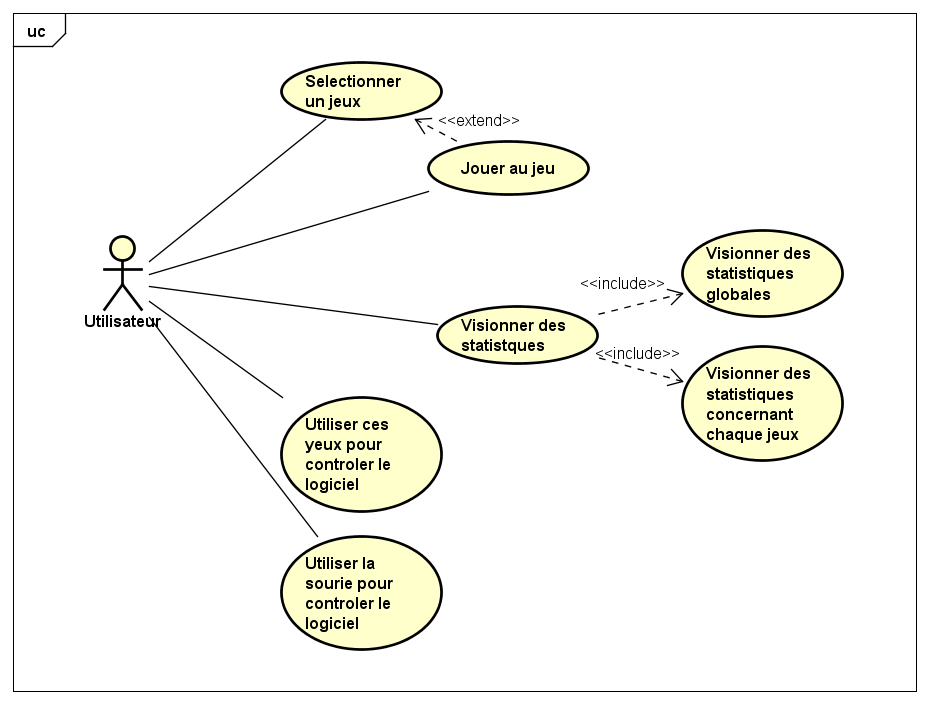
\includegraphics[width=13cm]{img/diagrammes/usecase.png}
    \caption{Diagramme des cas d'utilisation}
    \label{fig:use_case}
\end{figure}
\pagebreak

\paragraph{Description}
Comme vous pouvez le voir dans la figure~\ref{fig:use_case}, il n'existe qu'un utilisateur. Cet utilisateur a la possibilité de sélectionner un jeu parmi les jeux disponibles dans le menu. Lors de la sélection du jeu, il a la possibilité de jouer à ce jeu ou de visionner les statistiques relatives à ce jeu. Pour contrôler le logiciel, l'utilisateur à la possibilité d'utiliser la souris ou d'utiliser le dispositif d'eye tracking de l'entreprise Tobii. 

\paragraph{Cas d'utilisation nominal}
Dans le cadre d'une utilisation nominale du logiciel, l'utilisateur pourra effectuer les actions suivantes.

\begin{enumerate}
\item Dans un premier temps, l'utilisateur installe la barre Tobii. Il doit la positionner comme indiqué dans le manuel d'utilisation et réaliser la calibration de la barre.
\item Ensuite l'utilisateur lance le logiciel. Le logiciel démarre et affiche directement le menu principal. L'utilisateur peut alors quitter le jeu ou sélectionner un jeu. Pour effectuer une de ces actions, il faut que l'utilisateur positionne son regard sur le bouton souhaité pendant un certain temps.
\item Lorsque qu'un jeu est sélectionné, l'utilisateur va vouloir  jouer au jeu. Pour cela, il sélectionne le bouton "Jouer".
\item Dans le jeu, l'utilisateur suit les instructions spécifiques liées au jeu.
\item Lorsque qu'il souhaite arrêter, l'utilisateur clique sur le bouton "Quitter" disponible dans le jeu. Cela l'emmène directement au menu. Il peut également utiliser la croix rouge de fermeture des logiciels. Cela fermera définitivement le logiciel sans retour au menu.
\item Dans le menu,il peut à nouveau sélectionner un autre jeu (voir numéro 3) ou afficher les statistiques disponibles pour le jeu.
\item Dans le cas où l'utilisateur souhaite afficher les statistiques, il lui suffit de poser son regard sur le bouton prévu à cet effet.
\item Dans le menu des statistiques, l'utilisateur peut visionner des statistiques concernant le jeu. Il peut ensuite quitter via le bouton "Retour".
\item L'utilisateur est de nouveau dans le menu principal. Il peut sélectionner le bouton "Quitter" pour arrêter l'application.
\end{enumerate}

\paragraph{Cas d'utilisation exceptionnel}
Lorsque l'utilisateur va utiliser le programme il est possible que des problèmes surviennent ou qu'il effectue une mauvaise manipulation.

\textbf{Cas n°1}
\begin{enumerate}
\item L'utilisateur lance l'application sans avoir initialisé la barre Tobii
\item L'utilisateur installe la barre et la configure
\item L'utilisateur doit attendre le délai de reconnexion pour utiliser le logiciel
\item Retour au cas d'utilisation nominal
\end{enumerate}

\textbf{Cas n°2}
\begin{enumerate}
\item L'utilisateur lance l'application nominalement (initialisation de la barre Tobii et calibration réalisée)
\item Utilisation nominale du logiciel
\item Une déconnexion du port USB survient (erreur logiciel du système d'exploitation ou erreur humaine)
\item L'utilisateur rebranche le dispositif et attend le délai de reconnexion
\item Retour à un cas nominal
\end{enumerate}



\subsection{Définition des fonctions du système}
Dans cette partie nous définirons les différentes fonctions du système. Chacune de ces fonctions sera identifiée sommairement puis décrite plus en profondeur et de manière plus informatique.
\subsubsection{Contrôler le logiciel}
\paragraph{Identification de la fonction}
Le contrôle du logiciel est la fonction permettant d'utiliser les différents périphériques pour contrôler le jeu. Cette fonction est la plus importante du logiciel puisque c'est elle qui permettra de réaliser toutes les actions par la suite. Son efficacité est aussi très importante puisque la précision de cette fonction limitera la précision maximale autorisée dans le reste du programme.

\paragraph{Description de la fonction}
Cette fonctionnalité prend en charge l'utilisation de la barre de suivi visuel de Tobii. C'est elle qui va détecter si une barre est actuellement branchée sur l'ordinateur. Dans le cas où aucune barre n'est disponible, elle devra prendre en charge la souris pour permettre de naviguer entre les menus. Néanmoins, si un dispositif est branché, il prendra la main sur tout autres dispositifs.

\textbf{Précondition}
\begin{itemize}
\item Un dispositif de contrôle est branché. Cela peut être un dispositif d'eye tracking Tobii ou une souris. Ces dispositifs doivent être configurés et prêts à l'emploi, c'est à dire que les différents drivers nécessaires à leur fonctionnement sont installés
\end{itemize}

\textbf{Postcondition}
\begin{itemize}
\item La position du curseur est déterminée indépendamment du dispositif branché et  en boite noire pour le reste du logiciel.
\end{itemize}

\subsubsection{Sélectionner un jeu}
\paragraph{Identification de la fonction}
Cette fonction permet de choisir un jeu dans la liste des jeux disponibles. C'est donc une fonction principale du programme et une de celles que l'utilisateur verra en premier. Il est donc nécessaire de garantir l'ergonomie de cette fonction.

\paragraph{Description de la fonction}
Cette fonction est visible dans l'écran du menu. Elle met en place différents boutons permettant de sélectionner les jeux sous forme de tuiles (rectangles avec le nom du jeu et un visuel le représentant). La sélection d'une de ses tuiles permet de faire apparaître  les boutons "Jouer" et "Statistique". 

\textbf{Précondition}
\begin{itemize}
\item L'utilisateur doit disposer d'une application avec au moins un jeu installé.
\end{itemize}

\textbf{Postcondition}
\begin{itemize}
\item L'utilisateur peut accéder au jeu via le bouton "Jouer" ou au menu des statistiques via le bouton du même nom.
\end{itemize}

\subsubsection{Jouer au jeu}
\paragraph{Identification de la fonction}
Cette fonction est la plus importante du logiciel. Elle permet à l'utilisateur après avoir utilisé le menu et lancé le jeu d'y jouer.
\paragraph{Description de la fonction}
Lorsque l'utilisateur sélectionne un jeu dans le menu principal et souhaite y jouer, le jeu se lance et prend directement la main sur l'exécution du programme. Cette exécution est différente pour tous les jeux et n'est donc pas dépendante du logiciel. Néanmoins chaque jeu disposera de la fonctionnalité de contrôle du logiciel via le dispositif d'eye tracking (entre autre).

\textbf{Précondition}
\begin{itemize}
\item Le jeu doit avoir été implémenté au sein de l'application et bien configuré.
\end{itemize}

\textbf{Postcondition}
\begin{itemize}
\item L'utilisateur peut jouer à différents jeux utilisant les fonctionnalités d'eye tracking.
\end{itemize}

\subsubsection{Retourner au menu de sélection}
\paragraph{Identification de la fonction}
Cette fonctionnalité permet de quitter le jeu actuellement lancé afin de retourner à l'écran du menu. 

\paragraph{Description de la fonction}
Cette fonction met en place un bouton "Retour au menu principal" dans tous les jeux. Chaque jeu devra donc prévoir d'implémenter cette fonction.

\textbf{Précondition}
\begin{itemize}
\item Le jeu est lancé
\end{itemize}

\textbf{Postcondition}
\begin{itemize}
\item L'utilisateur est de nouveau dans le menu (écran de sélection des niveaux)
\end{itemize}

\subsubsection{Sauvegarder les statistiques}
\paragraph{Identification de la fonction}
Cette fonction permet de sauvegarder des statistiques durant l'exécution du programme. Cette fonctionnalité n'est pas une fonctionnalité principale mais peut être néanmoins considérée comme un plus. 
\paragraph{Description de la fonction}
Lors de chaque action de l'utilisateur dans un jeu nous sauvegardons cette action à des fins d'affichage de statistiques par la suite. Nous pouvons sauvegarder des statistiques pour  les mouvements du curseur ou à chaque victoire et défaite. Ces valeurs sont enregistrées dans l'application et seront utilisées par la fonction suivante pour les afficher.

\textbf{Précondition}
\begin{itemize}
\item L'application dispose d'un accès en écriture au système de fichier du système d'exploitation.
\end{itemize}

\textbf{Postcondition}
\begin{itemize}
\item Un fichier de statistiques est créé dans le répertoire du jeu.
\item Les actions de l'utilisateur sont enregistrées à des fins d'affichage.
\end{itemize}

\subsubsection{Afficher les statistiques}
\paragraph{Identification de la fonction}
Cette fonction permet d'afficher les statistiques récoltées lors de l'exécution du programme.
\paragraph{Description de la fonction}
L'utilisateur peut sélectionner l'affichage de statistiques dans le menu après avoir sélectionné un jeu. Les informations disponibles dans cette partie ne sont utiles que dans un but informatif. 

\textbf{Précondition}
\begin{itemize}
\item Des données doivent être disponibles pour le jeu sélectionné.
\end{itemize}

\textbf{Postcondition}
\begin{itemize}
\item Un affichage sous forme de texte est proposé à l'utilisateur.
\end{itemize}


\section{Spécification non fonctionnelles}
\subsection{Contraintes de fonctionnement}
\subsubsection{Performance}
Notre logiciel se doit d'être le plus performant possible. En effet, étant sous la forme d'un jeu vidéo toutes les pertes de performance (images par secondes) seront visibles et nuiront à l'expérience de l'utilisateur. C'est pourquoi nous souhaitons qu'une limite minimale d'au moins 30 images par secondes soit respectée. Cette limite représente le minima à respecter. La limite n'est néanmoins pas atteinte et le programme s'exécute actuellement au-delà de cette limite.
Le logiciel dispose aussi d'une limitation de performance que nous ne pouvons pas éviter. Il s'agit du taux de rafraîchissement du dispositif Tobii. Notre modèle nous permet de recevoir les informations de changement de positions des yeux à un intervalle de 120Hz à 1200Hz. Au-delà le rafraîchissement de l'application est inutile et ne ferait qu'augmenter les ressources utilisées.

\subsubsection{Maintenance et évolution du système}
\paragraph{Évolution}
Le programme rendu possède actuellement un ensemble de jeux. Cet ensemble est destiné à être étoffé par la suite. Nous avons donc mis en place un système permettant d'ajouter simplement des jeux à l'application. Le logiciel dispose actuellement de plusieurs composants simplifiants l'ajout de ses jeux par exemple, la mise à disposition  de boutons, de label, de compteurs etc. Chaque jeu qu'un développeur voudra ajouter pourra donc utiliser cette bibliothèque de composants pour développer son jeu. Pour l'intégration du jeu, il n'aura qu'à ajouter la création de son jeu à l'initialisation de l'application. Le logiciel intégrera ensuite ce jeu à la boîte en lui réservant un accès dans le menu. 

\paragraph{Maintenance}
Pour la maintenance, le logiciel dispose d'une fonctionnalité de journalisation permettant de connaître l'origine des problèmes qui pourraient survenir durant l'exécution du programme. Ces fichiers sont localisés dans le dossier \textit{log} de la release. 
En parallèle de ce système de journalisation, nous avons mis en place des documents de  maintenance. Ce document reprend les différentes parties du logiciel. Il indique les fonctionnalités présentes et comment elles sont implémentées. Ce document indique également les points critiques du logiciel (méthodes et composants essentiels). Il indique également les différentes bibliothèques que nous avons utilisées pour réaliser le logiciel. Il n'indique cependant pas comment utiliser en profondeur les bibliothèques. Pour cela, il faudra se référer à la documentation technique de la bibliothèque. 
Nous avons aussi documenté le programme le plus possible pour faciliter la lecture du code et sa compréhension. 

\chapter{Modélisation du logiciel}
\section{Diagramme de classe}
Lors de la phase d'analyse du problème nous avons émis plusieurs diagrammes de classes. Ces diagrammes nous ont permis de mettre en place l'architecture du programme. Nous avons essayé le plus possible d'adopter une architecture facilement maintenable et étendable. Nous avons aussi souhaité que l'architecture fasse abstraction des différentes bibliothèques que nous avons utilisées. Pour cela nous avons implémenté différentes classes empaquetant ces fonctionnalités. 


\pagebreak
\begin{figure}
    \centering
    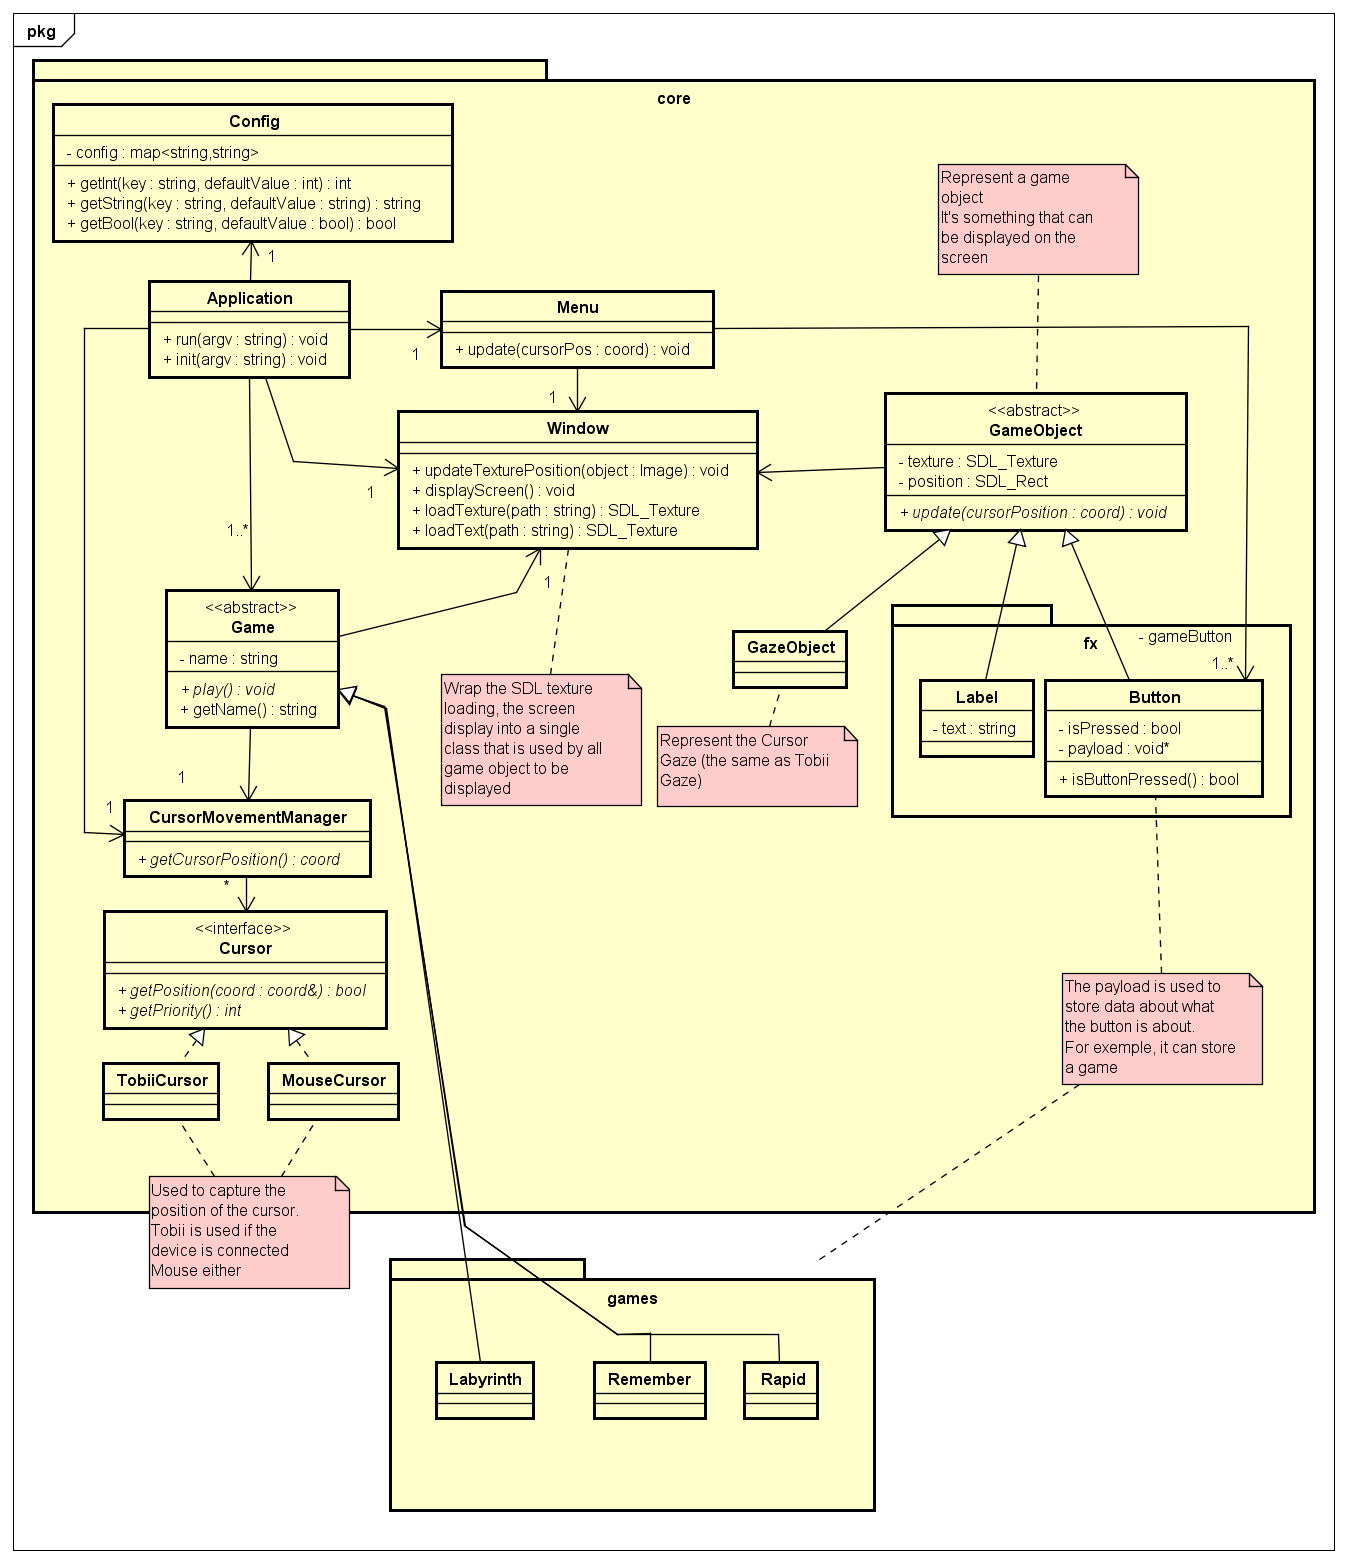
\includegraphics[width=15cm]{img/diagrammes/classDiag.png}
    \caption{Diagramme de classe}
    \label{fig:class_diag}
\end{figure}

Comme vous pouvez le voir dans la figure \ref{fig:class_diag} , nous avons décidé de découper notre logiciel en deux parties distincte (package). Ces deux parties sont \textit{core} et \textit{games}. La partie \textit{games} contient toutes les implémentations spécifiques à un jeu. Vous trouverez une partie détaillée plus en bas.

\paragraph{Le package \textit{core}}
Le package \textit{core} est la partie la plus importante du logiciel. C'est elle qui contient les classes permettant le bon fonctionnement de l'application. Nous pouvons le découper en plusieurs parties à la sémantique différente. 
Tout d'abord, nous pouvons trouver les classes \textit{Application}, \textit{Menu}, \textit{Window}, \textit{Config} et \textit{CursorMovementManager}. Ces classes ne sont pas vouées à posséder plusieurs instances dans le programme.  Elles servent principalement à l'affichage et au bon fonctionnement de l'application en général. 

\begin{itemize}
\item La classe \textit{Application} permet de lancer l'application. C'est elle qui va instancier les différentes parties du logiciel. Pour plus de détails veuillez vous référer à la partie Fonctionnement du système (\autoref{sec:fonc_init})
\item La classe \textit{Window} est une classe permettant de s'abstraire de la bibliothèque graphique que nous avons utilisée. Cette classe regroupe les différentes fonctionnalités pour créer des textures (images en mémoire) et de les afficher aux positions souhaitées. Une seule instance de cette classe est créée dans tout le programme et est transmise à tous les objets ayant besoin de  s'afficher à l'écran. 
\item La classe \textit{Config} permet de charger en mémoire les différentes configuration souhaitées par l'utilisateur. Le fichier de configuration se trouve dans le dossier \textit{ressource} du programme et se nomme \textit{config.ini}. Ce fichier se décompose en plusieurs instructions d'égalités du type \textit{key=value}. Dans le programme il sera possible de récupérer chacune des valeurs (entière, booléenne ou en chaîne de caractère) sauvegardées dans le fichier de configuration via sa clé. 
\item La classe {Menu} est une classe utilitaire permettant d'implémenter la logique du menu et de simplifier le code de la classe \textit{Application}.
\item La classe \textit{CursorMovementManager} est une classe un peu spéciale puisqu'elle permet de définir et de récupérer la position du curseur. Un curseur (ou \textit{Cursor} dans le diagramme) est une classe permettant de définir la position du regard de l'utilisateur. Il peut soit s'agir de la  souris (\textit{MouseCursor}) ou de l'emplacement du regard récupéré grâce au dispositif Tobii (\textit{TobiiCursor}). Nous expliciterons le fonctionnement de la classe \textit{TobiiCursor} plus en détails en bas (\autoref{sec:fonc_tobii})
\end{itemize}

Le package {core} met aussi à disposition différentes classes permettant de simplifier le développement des jeux et du logiciel en général. Dans ces classes nous pouvons trouver le \textit{GameObject} et ces sous-classes \textit{Label} et \textit{Button}. La classe \textit{GameObject} représente un objet du jeu pouvant s'afficher à l'écran. Elle possède une méthode \textit{update} permettant de mettre à jour l'état de l'objet et de mettre à jour l'affichage. 
Les classes \textit{Button} et \textit{Label} sont des utilitaires permettant de créer des boutons et d'afficher du texte à l'écran.

\pagebreak
\paragraph{Le package \textit{games}}
Ce package contient les différentes classes en rapport avec les jeux. Nous pouvons voir dans le diagramme suivant (\autoref{fig:class_pk_games}) l'architecture du package \textit{games}. Elle met en place différents sous-packages pour chaque jeu et leurs classes.  Par exemple le jeu \textit{Remember} (jeu de mémorisation) possède différentes \textit{Cases} symbolisant les boutons à cliquer dans l'ordre. Il possède également des \textit{GameObject} pour afficher ces mêmes cases mais avec un texte symbolisant le numéro de la case.

\begin{figure}
    \centering
    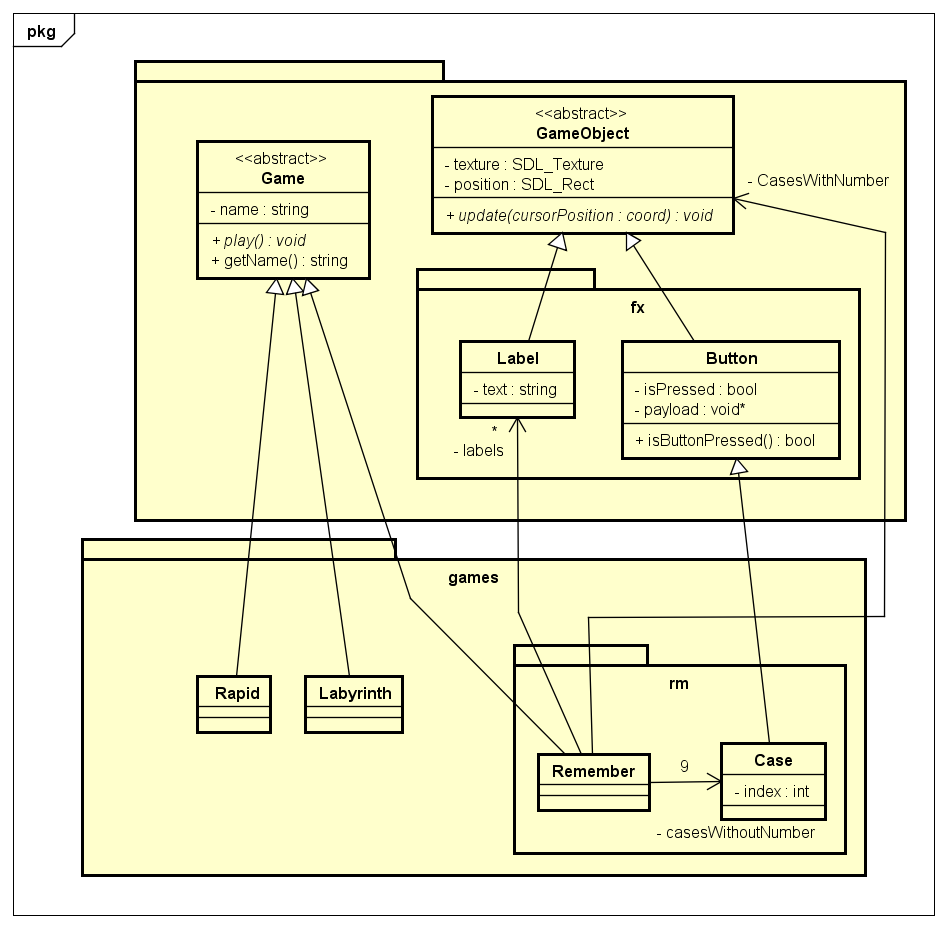
\includegraphics[width=13cm]{img/diagrammes/classPkGames.png}
    \caption{Diagramme de classe du package games}
    \label{fig:class_pk_games}
\end{figure}


\section{Fonctionnement du système}
\subsection{Fonctionnement global}
Pour expliciter le fonctionnent globale de l'application nous avons réalisé un diagramme d'activité. Dans la boucle principale du jeu (Mise à jour - Rafraîchissement - Décision) l'utilisateur a plusieurs choix : Il peut sélectionner un jeu, lancer le jeu ou tout simplement quitter l'application.
Lors de la sélection d'un jeu, le bouton "Jouer" apparaît. Il sera donc possible de cliquer dessus pour lancer le jeu. Lorsque 'un jeu est lancé, il prend le contrôle de l'application. C'est donc à lui de redéfinir les différentes actions et méthodes de rafraîchissement qui lui sont propres.
\begin{figure}
    \centering
    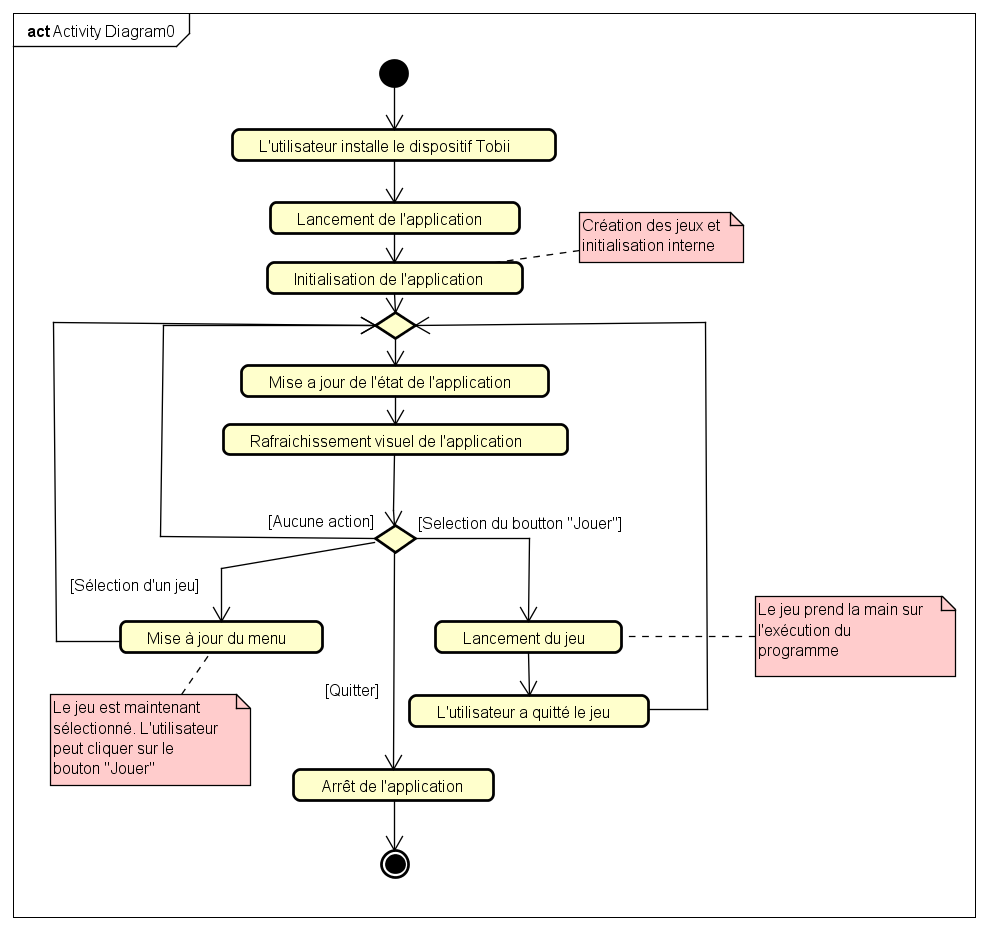
\includegraphics[width=15cm]{img/diagrammes/ActivityFoncPrincipal.png}
    \caption{Diagramme d'activité du programme}
    \label{fig:activityDiag}
\end{figure}
\subsection{Initialisation du programme}
\label{sec:fonc_init}
Lors du lancement du programme, plusieurs actions d'initialisation sont effectuées dans la méthode \textit{init()} de la classe \textit{Application}. Nous avons rédigé un diagramme de séquence pour expliciter son fonctionnement (cf \autoref{fig:seq_init}). 

\begin{figure}
    \centering
    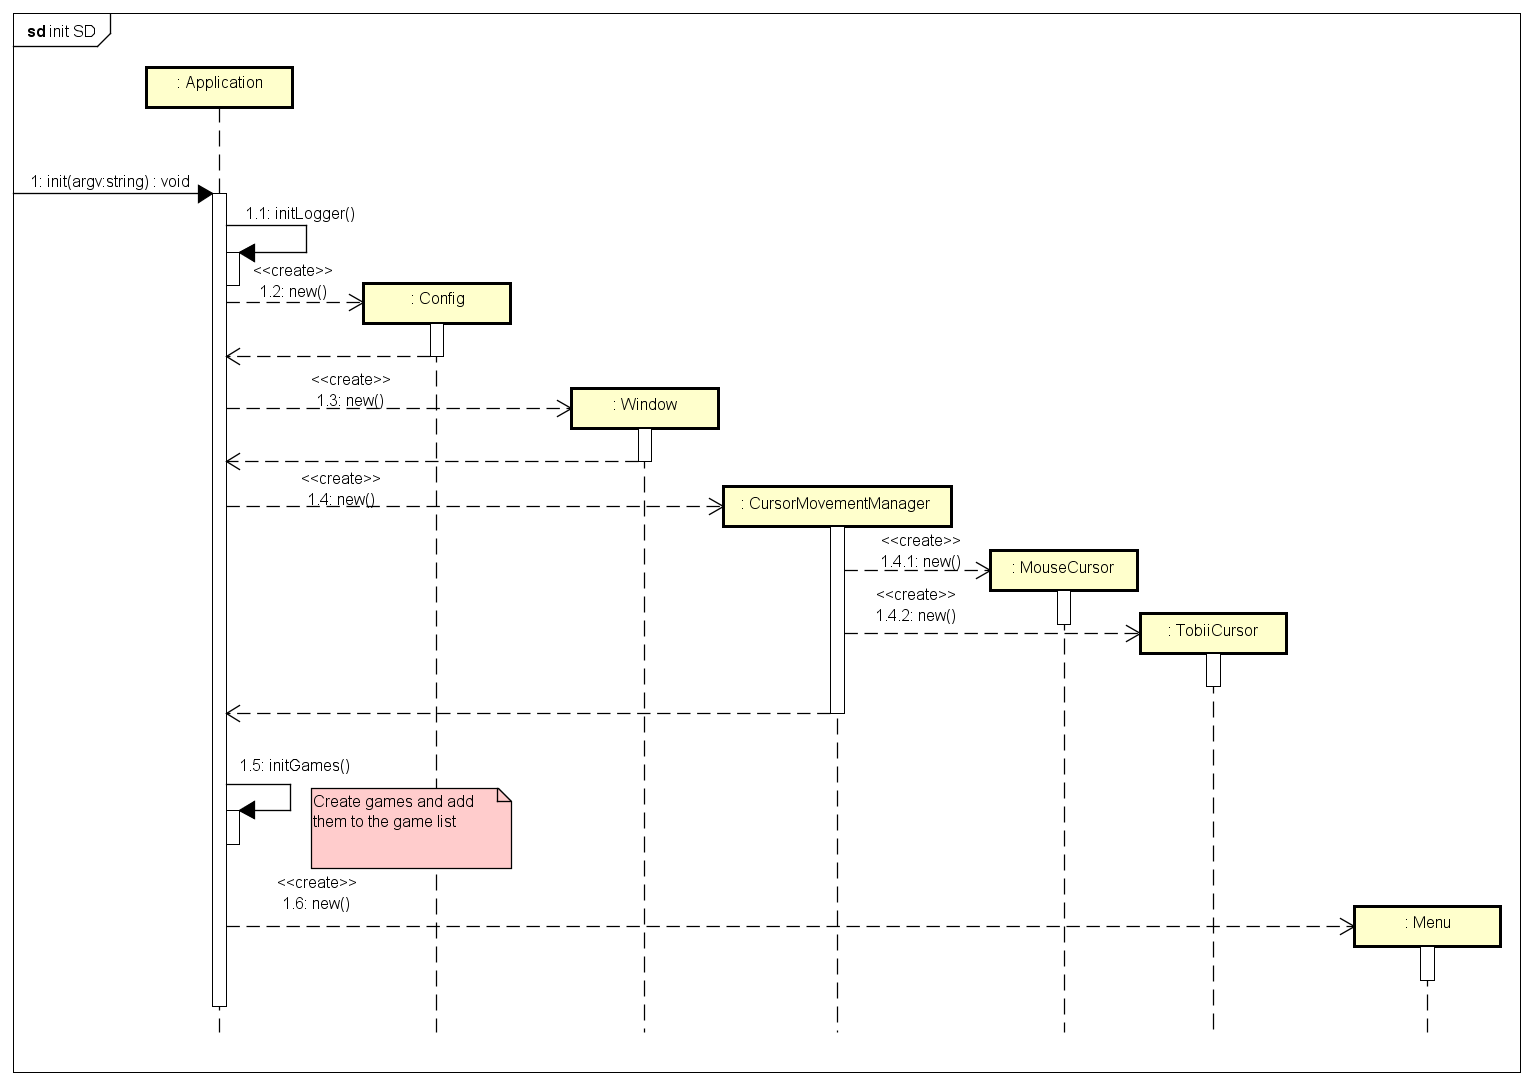
\includegraphics[width=15cm]{img/diagrammes/seqInit.png}
    \caption{Diagramme de séquence de l'initialisation de l'application}
    \label{fig:seq_init}
\end{figure}

Dans ce diagramme nous pouvons voir le cycle de vie de la méthode \textit{init()} de l'application. Cette méthode a pour but de créer les différents composants du logiciel. Elle va donc prioritairement créer le système de journalisation. C'est lui qui permettra de débugguer facilement l'application. Il est donc nécessaire de l'instancier au début. Vient ensuite la lecture de la configuration de l'utilisateur. Cette lecture est nécessaire pour charger les différentes configurations souhaitées par l'utilisateur (par exemple la taille de la fenêtre, la durée du temps nécessaire pour considérer un clique sur un bouton etc).
L'application peut ensuite créer les différentes autres parties comme les curseurs et le Menu.
Les jeux sont aussi instanciés dans cette méthode. Il suffit pour cela d'ajouter à la liste des jeux connus par l'application le jeu souhaité. Les curseurs sont créés via le \textit{CursorMovementManager} et le fonctionnement plus en détail est explicité ici \autoref{sec:fonc_cursors}.

\subsection{Fonctionnement des curseurs}
\label{sec:fonc_cursors}
Comme nous l'avons dit plus haut, les curseurs sont les objets permettant de récupérer l'emplacement du regard de l'utilisateur. Pour effectuer ce traitement nous avons souhaité pouvoir utiliser la souris et le dispositif Tobii. La souris (\textit{MouseCursor}) est présente uniquement à des fins de tests (ne possédant pas deux barres nous avons souhaitez pouvoir utiliser le logiciel quand même). La création des curseurs est réalisée par la classe \textit{CursorMovementManager}, c'est donc elle qui gère les curseurs. 
Nous pouvons voir le fonctionnement des curseurs dans le diagramme suivant (\autoref{fig:seq_Cursor})
\pagebreak
\begin{figure}
    \centering
    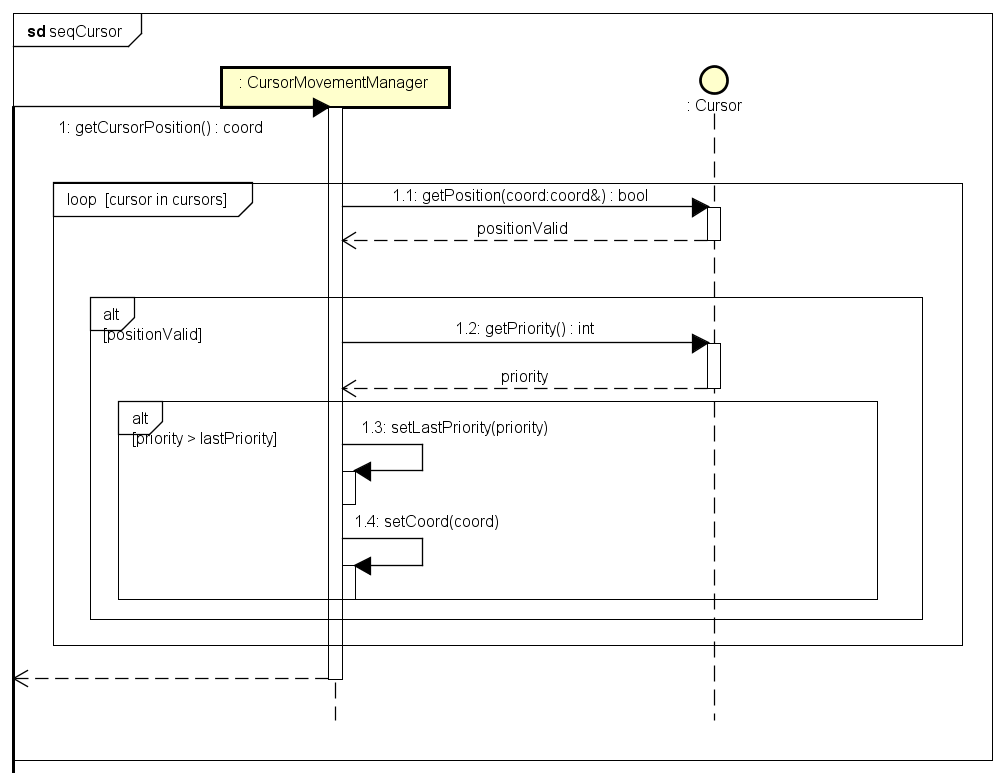
\includegraphics[width=15cm]{img/diagrammes/seqCursor.png}
    \caption{Diagramme de séquence du fonctionnement des curseurs}
    \label{fig:seq_Cursor}
\end{figure}
Les curseurs fonctionnent avec un dispositif de priorité et de validité. La priorité d'un curseur permet de définir quelle valeur choisir lorsque plusieurs valeurs sont disponibles. Par exemple dans le cas où un dispositif Tobii et une souris sont branchés, le curseur gérant la barre Tobii aura plus de priorité que la souris. Chacune des demandes de récupération de position retourne un booléen permettant de savoir si la position est valide. Par exemple si aucun dispositif Tobii n'est branché, son curseur indiquera \textit{false} pour ne pas utiliser la valeur retournée. A la fin, seule la valeur avec la priorité la plus élevée et valide sera gardée. 

\subsection{Fonctionnement la classe \textit{TobiiCursor}}
\label{sec:fonc_tobii}
Le fonctionnement de la classe \textit{TobiiCursor} est particulière et dépend des évènements externes. En effet, cette classe permet d'interagir avec l'API de la barre Tobii et cette API peut retourner différentes erreurs propres à l'utilisation de la barre. Il est aussi possible qu'un cas exceptionnel de cas d'utilisation survienne (\autoref{fig:use_case}). Nous pouvons donc lister les différentes erreurs possibles suivantes : 
\begin{itemize}
    \item La barre n'est pas branchée lors du lancement de l'application
    \item Une déconnexion de la barre survient pendant l'exécution
    \item Les données retournées par l'API Tobii sont marquées comme invalides (ex : l'utilisateur ne regarde plus l'écran)
\end{itemize}
Ces 3 cas correspondent à une gestion d'erreurs différentes qu'il faut gérer pour garantir l'efficacité de l'application. Le fonctionnement du curseur et son initialisation peuvent être résumés comme tel :

\begin{algorithm}
\SetAlgoLined
\DontPrintSemicolon
\SetKwFunction{Fun}{Initalize}
\Fun{}{
\BlankLine
    $api \gets tobii\_api\_create()$\;
    $device\_urls \gets tobii\_enumerat\_local\_device\_urls(api)$\;
    \uIf{$device\_urls$ \textbf{is empty}}{
      print error\;
    }
    \Else{
        $device\_url \gets device\_urls[0]$\;
    	$device \gets tobii\_device\_create(api, device\_url)$\;
    	$tobii\_gaze\_point\_subscribe(device)$\;
    }
}
\caption{TobiiCursor Initialisation}
\label{algo:init_tobiiCursor}
\end{algorithm}

\begin{algorithm}
\SetAlgoLined
\DontPrintSemicolon
\SetKwFunction{Fun}{Cursor::getCursorPosition}
\Fun{$coordinates$}{
\BlankLine
    \lIf{$device$ \textbf{not initialized}}{
      $init\_device(device)$\;
    }
    
    $tobii\_gaze\_point\_data \gets tobii\_device\_process\_callbacks(device)$\;
    
    \uIf{$device$ \textbf{is disconnected}}{
         $reconnect\_device(device)$\;
         \Return $false$\;
    }
    \uElseIf{$tobii\_gaze\_point\_data$ \textbf{is not valid}}{
        \Return $false$\;
    }

    $coordinates \gets tobii\_gaze\_point\_data$\;
    \Return $true$\;
}
\caption{Fonctionnement de la méthode \textit{getCursorPosition} de la classe \textit{TobiiCursor}}
\label{algo:getpos_tobiiCursor}
\end{algorithm}

\pagebreak
Pour mieux comprendre les types de retours et les paramètres, veuillez vous référer à \autoref{fig:class_diag} et \autoref{sec:fonc_cursors}.

\paragraph{Initialisation}
Tout d'abord, l'application va initialiser un composant permettant d'utiliser l'API Tobii. Ce composant est initialisé en utilisant un appel au SDK de Tobii \cite{tobiiApi}. 

Il faut ensuite localiser et initialiser le dispositif Tobii branché au PC. Pour cela le SDK de Tobii met à disposition une API permettant de lister les dispositifs actuellement branchés (\textit{tobii\_enumerate\_local\_device\_url(...)} ). Cette API nous donne accès au URL des dispositifs (l'URL utilise un protocole spécial et unique à Tobii). 

Grâce à cette URL nous pouvons créer un composant Tobii (\textit{tobii\_device\_t}). Nous allons ensuite abonner ce composant aux données du \textit{point de regard} (en Anglais \textit{Gaze point}) de l'utilisateur. Cet abonnement permet par un système de paterne Observateur de nous notifier lorsqu'une nouvelle donnée de pointage est disponible.

Si aucun dispositif n'est branché lors de l'initialisation, le composant du dispositif Tobii n'est pas initialisé et il faudra donc tenter de l'initialiser par la suite. Cette initialisation sera réalisée au même endroit que la gestion de la déconnexion mais n'effectuera pas le même traitement.

\paragraph{Détection d'une déconnexion}
Lorsqu'une déconnexion survient, il nous est impossible de récupérer les données de la position du regard. Le SDK Tobii nous indique le problème suite à l'appel de la fonction \textit{tobii\_device\_process\_callbacks(device)}. Lorsque nous interceptons cette erreur nous faisons appel à la fonction de reconnexion disponible dans le SDK \textit{tobii\_device\_reconnect(device)}. Cette fonction va tenter de reconnecter le composant. 

Lors de nos tests nous avons remarqué une perte de performance dû à l'appel de cette fonction. En effet après investigation, il s'est avéré que la fonction lançait un Thread pour chaque appel. Nous avons donc décidé de mettre en place un timer pour limiter le nombre de tentatives de reconnexion dans le temps. La durée de ce timer peut être modifiée dans le fichier de configuration.

\paragraph{Détection d'un erreur de lecture}
Lorsque nous récupérons les données de position fournies par l'API Tobii nous pouvons faire fasse à des positions invalides. Ce cas peut se présenter pour diverses raisons. Par exemple lorsque l'utilisateur ne regarde plus l'écran ou qu'un élément se trouve entre la barre Tobii et l'utilisateur. Etant donné que les données reçues sont invalides nous ne pouvons pas les utiliser et nous indiquons donc au \textit{CursorMovemementManager} (\autoref{fig:class_diag}) qu'il ne faut pas qu'il prenne en compte ce curseur.

\subsection{Mockups de l'application}
\label{sec:mockups}
Avant de réaliser l'application nous avons réalisé des mockups pour avoir une ligne directrice lors du développement. Ces mockups regroupent les différentes pages de l'application ainsi que les pages associées aux jeux. 
Nous avons essayé de mettre en place une interface simple et épurée pour qu'elle soit la plus intuitive possible afin de permettre à tout type d'utilisateur de prendre en main le logiciel facilement. Les boutons de notre interface devront être assez grands pour que les problèmes de précision du dispositif Tobii ne soient pas un problème pour notre application. Vous pouvez voir les visuels dans les figures suivantes \autoref{fig:mockup_mainmenu}, \autoref{fig:mockup_memo}, \autoref{fig:mockup_fast} et \autoref{fig:mockup_maze}.

\begin{figure}
    \centering
    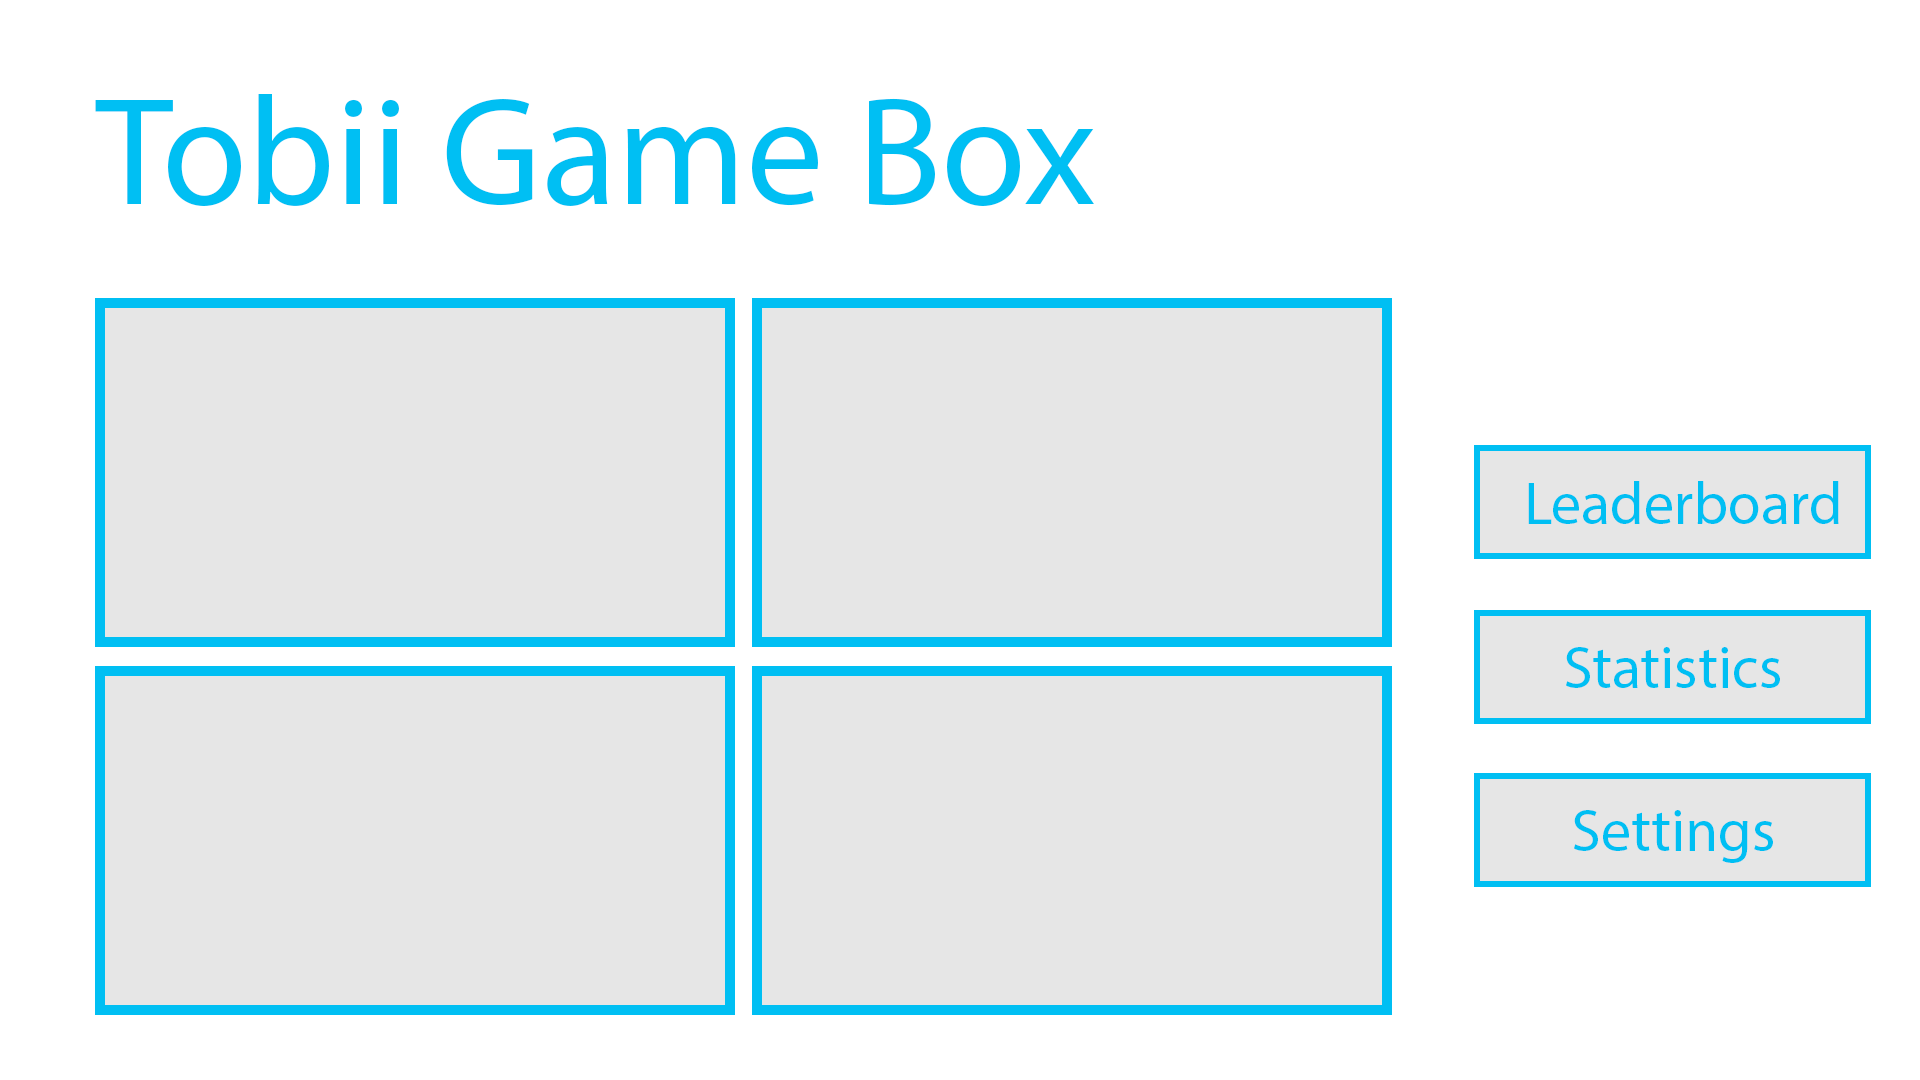
\includegraphics[width=15cm]{img/mockups/MainMenu.png}
    \caption{Mockup du menu principal}
    \label{fig:mockup_mainmenu}
\end{figure}

\begin{figure}
    \centering
    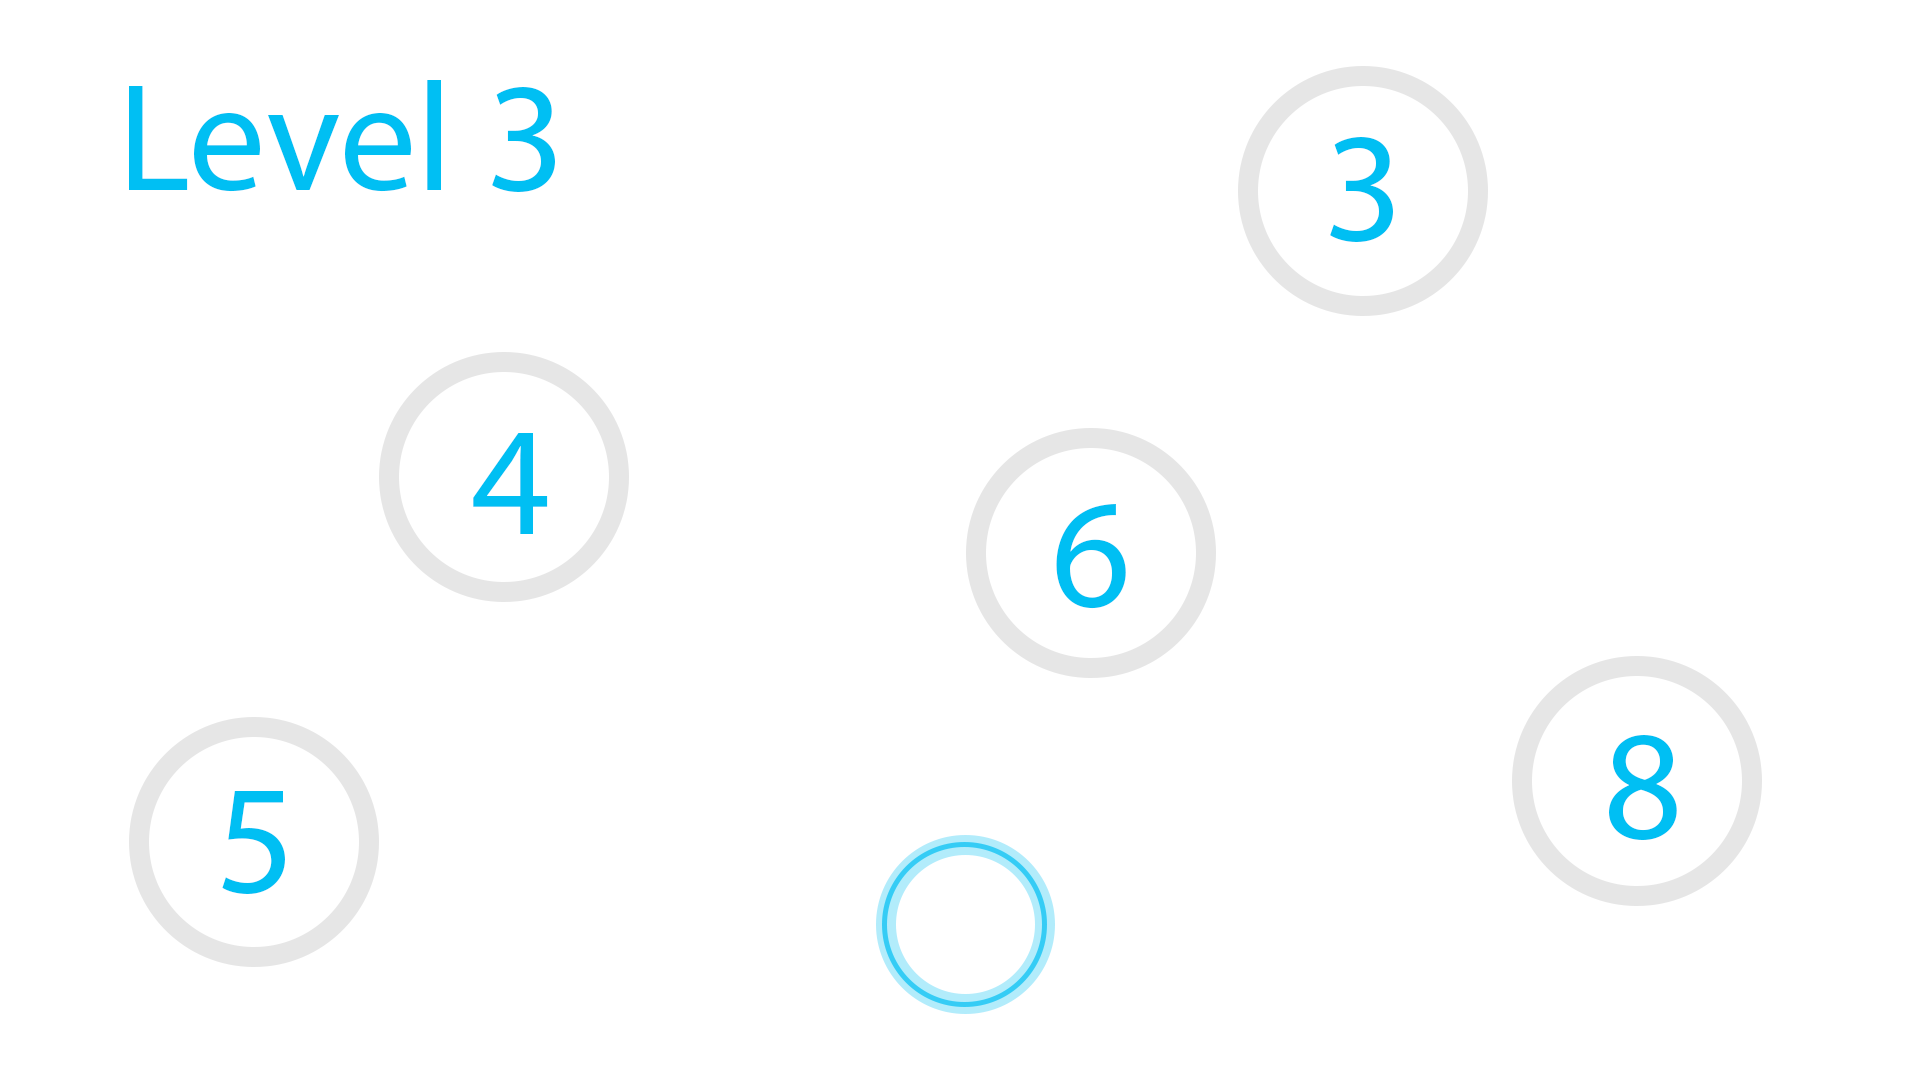
\includegraphics[width=15cm]{img/mockups/Remember(LvL3).png}
    \caption{Mockup du jeu de mémorisation}
    \label{fig:mockup_memo}
\end{figure}

\begin{figure}
    \centering
    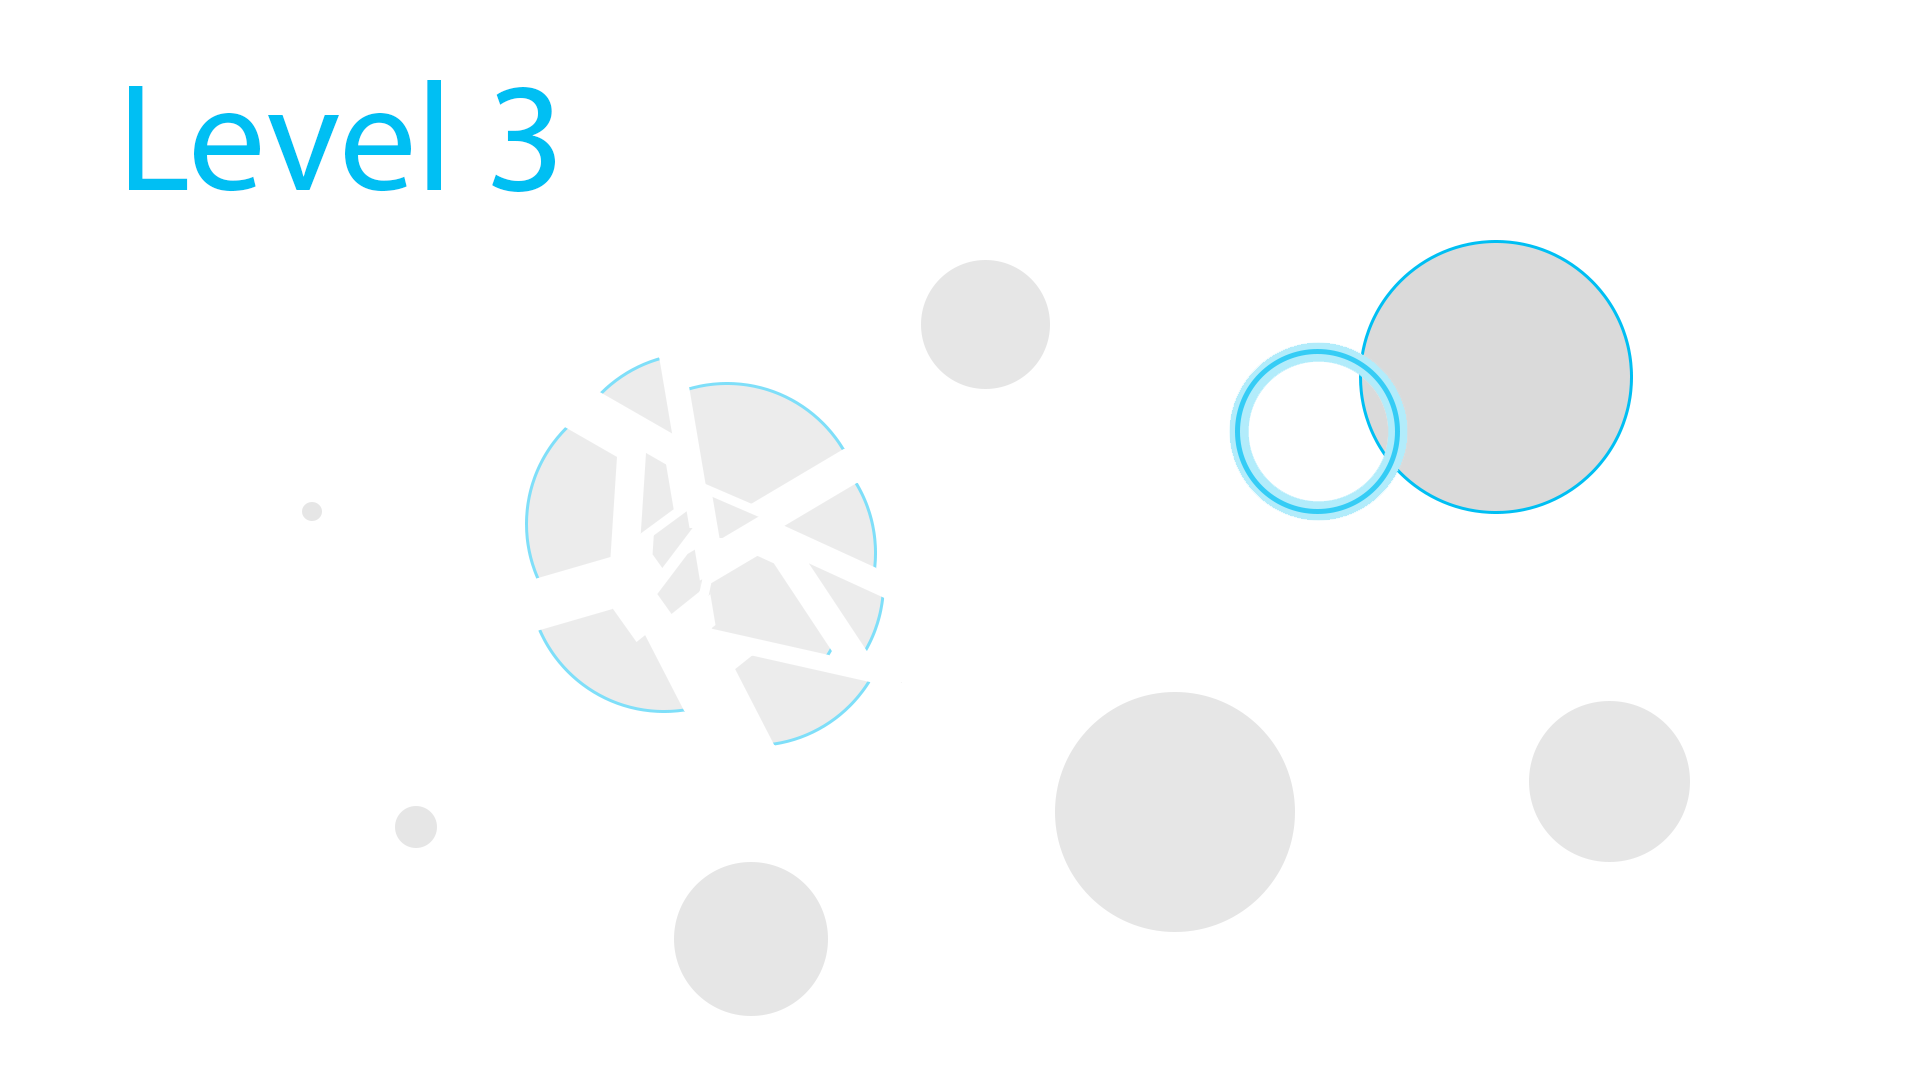
\includegraphics[width=15cm]{img/mockups/RapideEyeMovement.png}
    \caption{Mockup du jeu de rapidité}
    \label{fig:mockup_fast}
\end{figure}

\begin{figure}
    \centering
    
\includegraphics[width=15cm]{img/mockups/Maze.png}
    \caption{Mockup du jeu du labyrinthe}
    \label{fig:mockup_maze}
\end{figure}

\chapter{Implémentation et Tests}
\section{Implémentation}
L'implémentation du logiciel a été réalisée en C++ en utilisant plusieurs bibliothèques :
\begin{itemize}
\item SDL version 2 (Simple DirectMedia Layer \cite{sdl2}) est une bibliothèque permettant de gérer l'aspect graphique d'une application. Elle permet aussi de gérer les entrées des périphériques comme par exemple la souris ou le clavier. Nous avons ajouté des dépendances supplémentaires à cette bibliothèque pour nous faciliter le développement. 
\begin{itemize}
\item SDL Image \cite{sdl2_image}, cette ajout à la SDL permet de gérer plus facilement le chargement des images au sein de l'application en permettant de charger les images au format png, jpg, gif etc. Normalement, la SDL ne permet de charger que les images au format BMP.
\item SDL TTF \cite{sdl2_ttf}, cette ajout permet d'afficher du texte à l'écran. Elle permet de convertir des chaînes de caractères en images affichables à l'écran. 
\item SDL Mixer \cite{sdl2_mixer}, cette ajout à la SDL permet de gérer l'audio d'une application en mettant à disposition des moyens de charger des fichiers mp3 et de les lire dans l'application.
\end{itemize}
\item SPDLOG \cite{spdlog}. Cette bibliothèque permet de générer des fichiers de journalisation et de formater les sorties console. Cette bibliothèque est utile pour le développement de l'application et la recherche de bugs. Elle n'est néanmoins pas visible pour l'utilisateur. 
\item Le stream SDK Tobii \cite{tobiiApi}. Cette bibliothèque nous donne accès aux différentes fonctionnalités du dispositif de suivi oculaire Tobii. Elle est rédigée en C++ avec des instructions bas niveau (récupération de la position des yeux et de la tête).
\end{itemize}

Pour réaliser l'implémentation du programme nous avons utilisé l'EDI Visual Studio 2017. Les fichiers de configuration du projet sont disponibles dans le dossier du rendu. Nous avons également généré un fichier CMakeLists.txt permettant de générer le programme via l'utilitaire cmake. 

L'implémentation du projet a été réalisée à la suite de la phase de conception. Néanmoins, certaines retouches ont été effectuées au cours du développement principalement au niveau des ajouts de fonctionnalités que nous n'avions pas anticipées et qui se sont révélées utiles pour la suite du projet. 

\section{Déroulement du projet}
Le projet a commencé fin septembre début octobre. Durant les premières semaines nous avons réalisé différents documents et diagrammes nous permettant d'avancer par la suite. Au début nous avions également sélectionné le langage de programmation Python avec différentes bibliothèques (par exemple une bibliothèque graphique etc.). Malheureusement, Tobii n'indique pas clairement sur son site que les SDK "pro" qui mettent à disposition le langage Python sont payants. Nous n'avions pas eu cette information et après discussion, l'entreprise Tobii nous a proposé une licence à 2400€. Il nous était donc impossible d'utiliser le langage Python malgré le fait que nous avions déjà commencé à programmer dans ce langage. 
	Nous avons donc dû recommencer le projet fin novembre (cf. les comptes rendus ci-dessous). 
    
\section{État de l'avancement du projet}
Au jour du rendu, le projet n'est pas totalement fini. En effet, la perte de temps causé par les problèmes rencontrés au  début du projet nous ont ralenti et nous n'avons pas pu réaliser tout ce que nous souhaitions. Nous avons tout de même programmé la plupart des fonctionnalités que nous voulions. Notre projet contient donc les fonctionnalités suivantes :
\begin{itemize}
\item Un jeu totalement fonctionnel (Jeu de mémoire)
\begin{itemize}
\item Un système de niveaux avec des difficultés progressives
\item Une génération de niveau aléatoire
\end{itemize}
\item Un système de statistiques pour chaque jeu
\item Un menu totalement fonctionnel
\begin{itemize}
\item Possibilité de jouer à n'importe quel jeu ajouté
\item Possibilité de stocker et de visionner des statistiques pour chaque jeu
\item Possibilité de quitter l'application
\end{itemize}
\item Un système de configuration unique pour tous les composants du système
\item La gestion des sons et de la musique de l'application
\end{itemize}

Cependant, il nous manque certaines fonctionnalités que nous avions prévu de mettre en place. Nous n'avons en effet pas pu implémenter tous les jeux que nous souhaitions. Nous n'avons donc pas pu créer le jeu du labyrinthe et le jeu de rapidité. Cela peut s'expliquer par notre souhait de vouloir produire un jeu complet et non plusieurs jeux non finis et non soignés. Ce retard peut aussi s'expliquer par notre volonté de produire plusieurs composants qui ne sont pas indispensables au projet mais permettant néanmoins de faciliter le développement des jeux. Dans ces composants nous pouvons citer la classe \textit{GameObject} et ces classes héritées (\textit{Label} et \textit{Button}). 

\paragraph{Visuel de l'application}
A la suite du développement, l'application que nous avons développée diverge un peu des mockups que nous avions initialement créés. Vous pouvez voir les différents pages de l'application dans les figure \autoref{fig:screenshot_main_menu}, \autoref{fig:screenshot_game_expli}, \autoref{fig:screenshot_game}, \autoref{fig:screenshot_game_invisible}, \autoref{fig:screenshot_statistics}

\begin{figure}
    \centering
    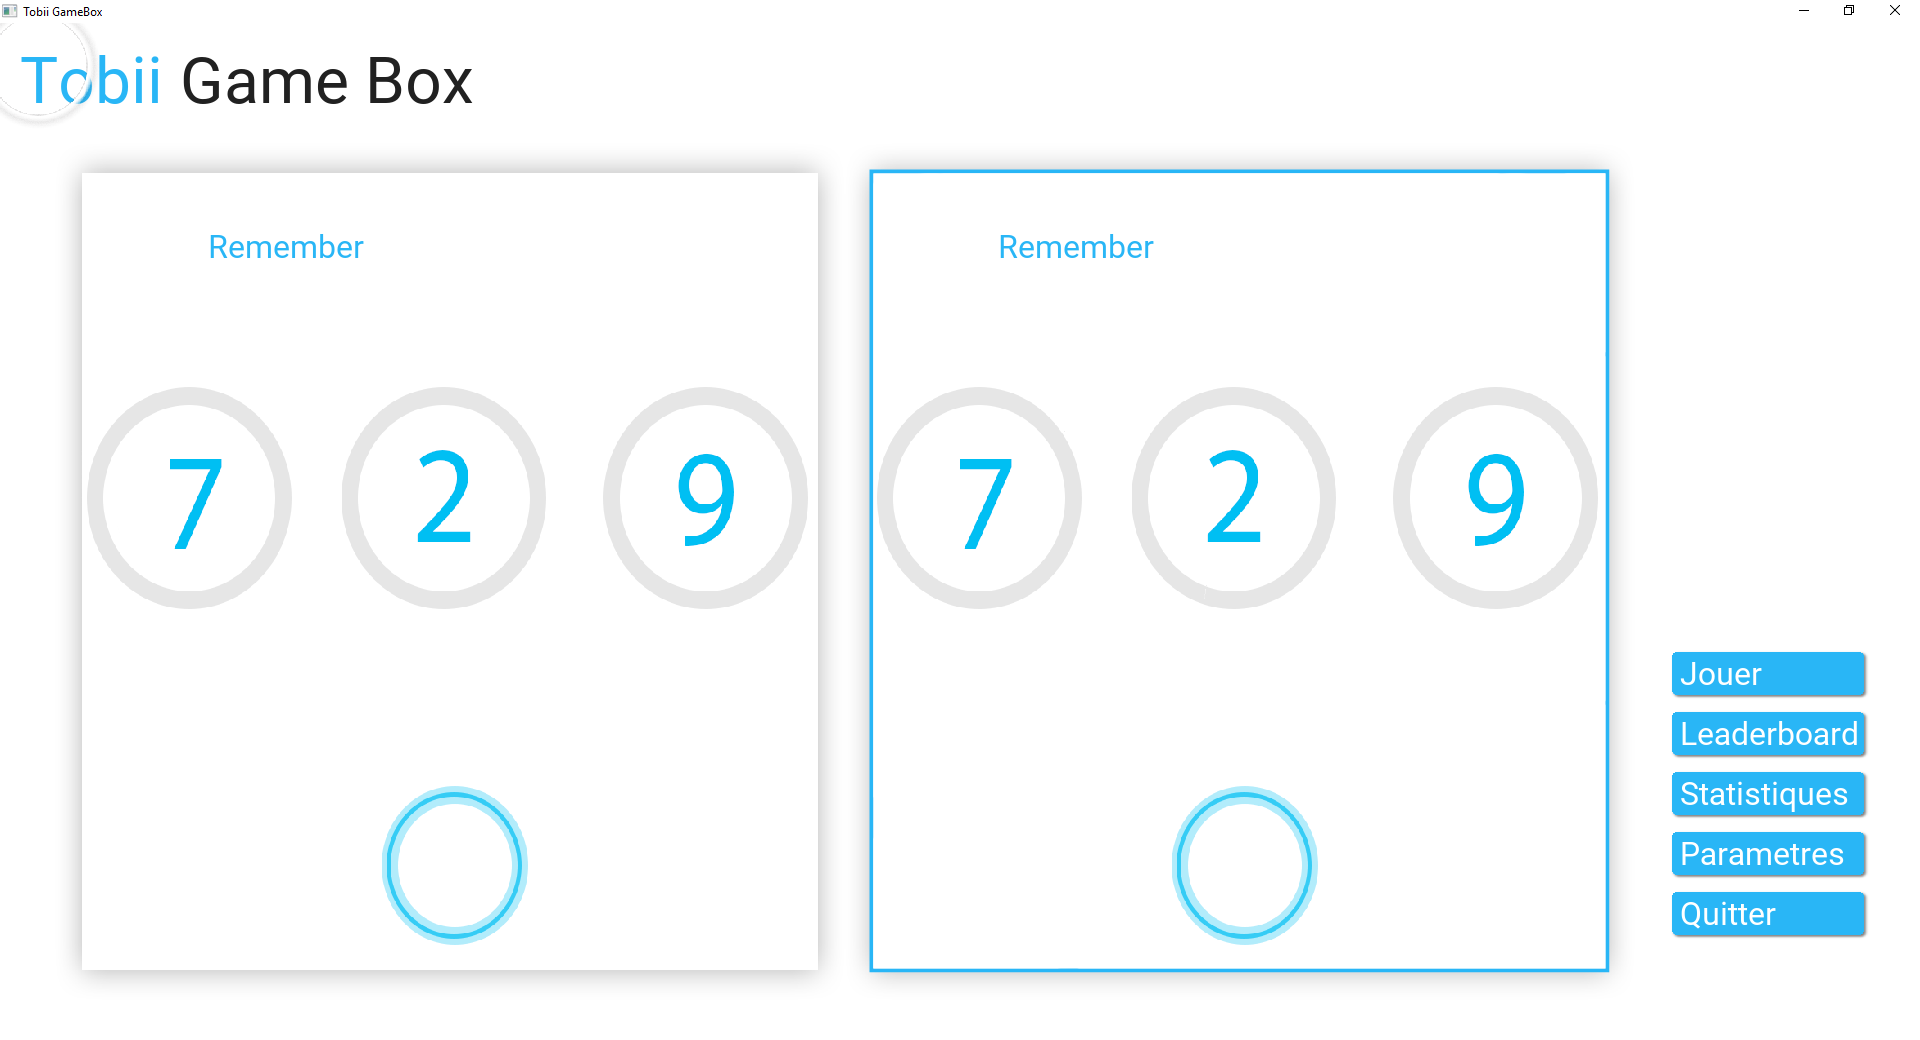
\includegraphics[width=15cm]{img/screenshots/menu_principal.PNG}
    \caption{Menu principal du jeu}
    \label{fig:screenshot_main_menu}
\end{figure}

\begin{figure}
    \centering
    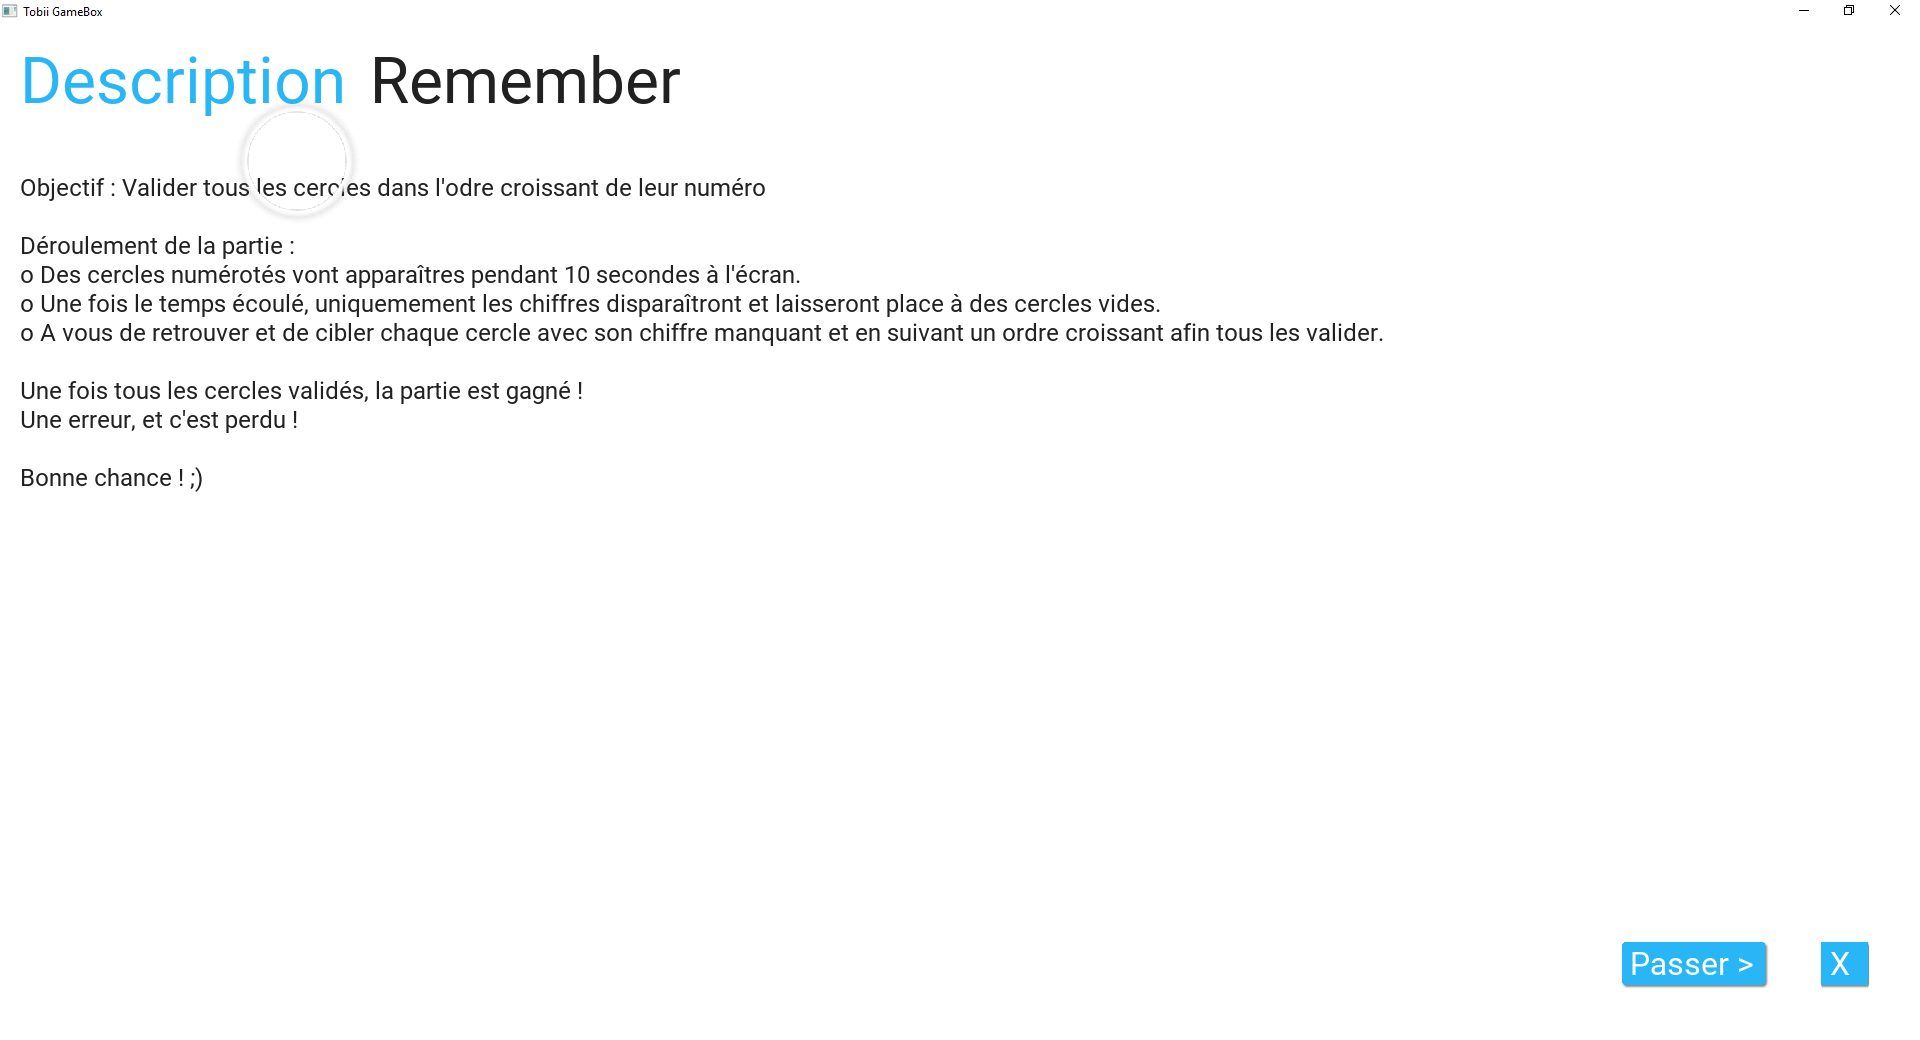
\includegraphics[width=15cm]{img/screenshots/jeu_explication.PNG}
    \caption{Menu d'explication du jeu}
    \label{fig:screenshot_game_expli}
\end{figure}

\begin{figure}
    \centering
    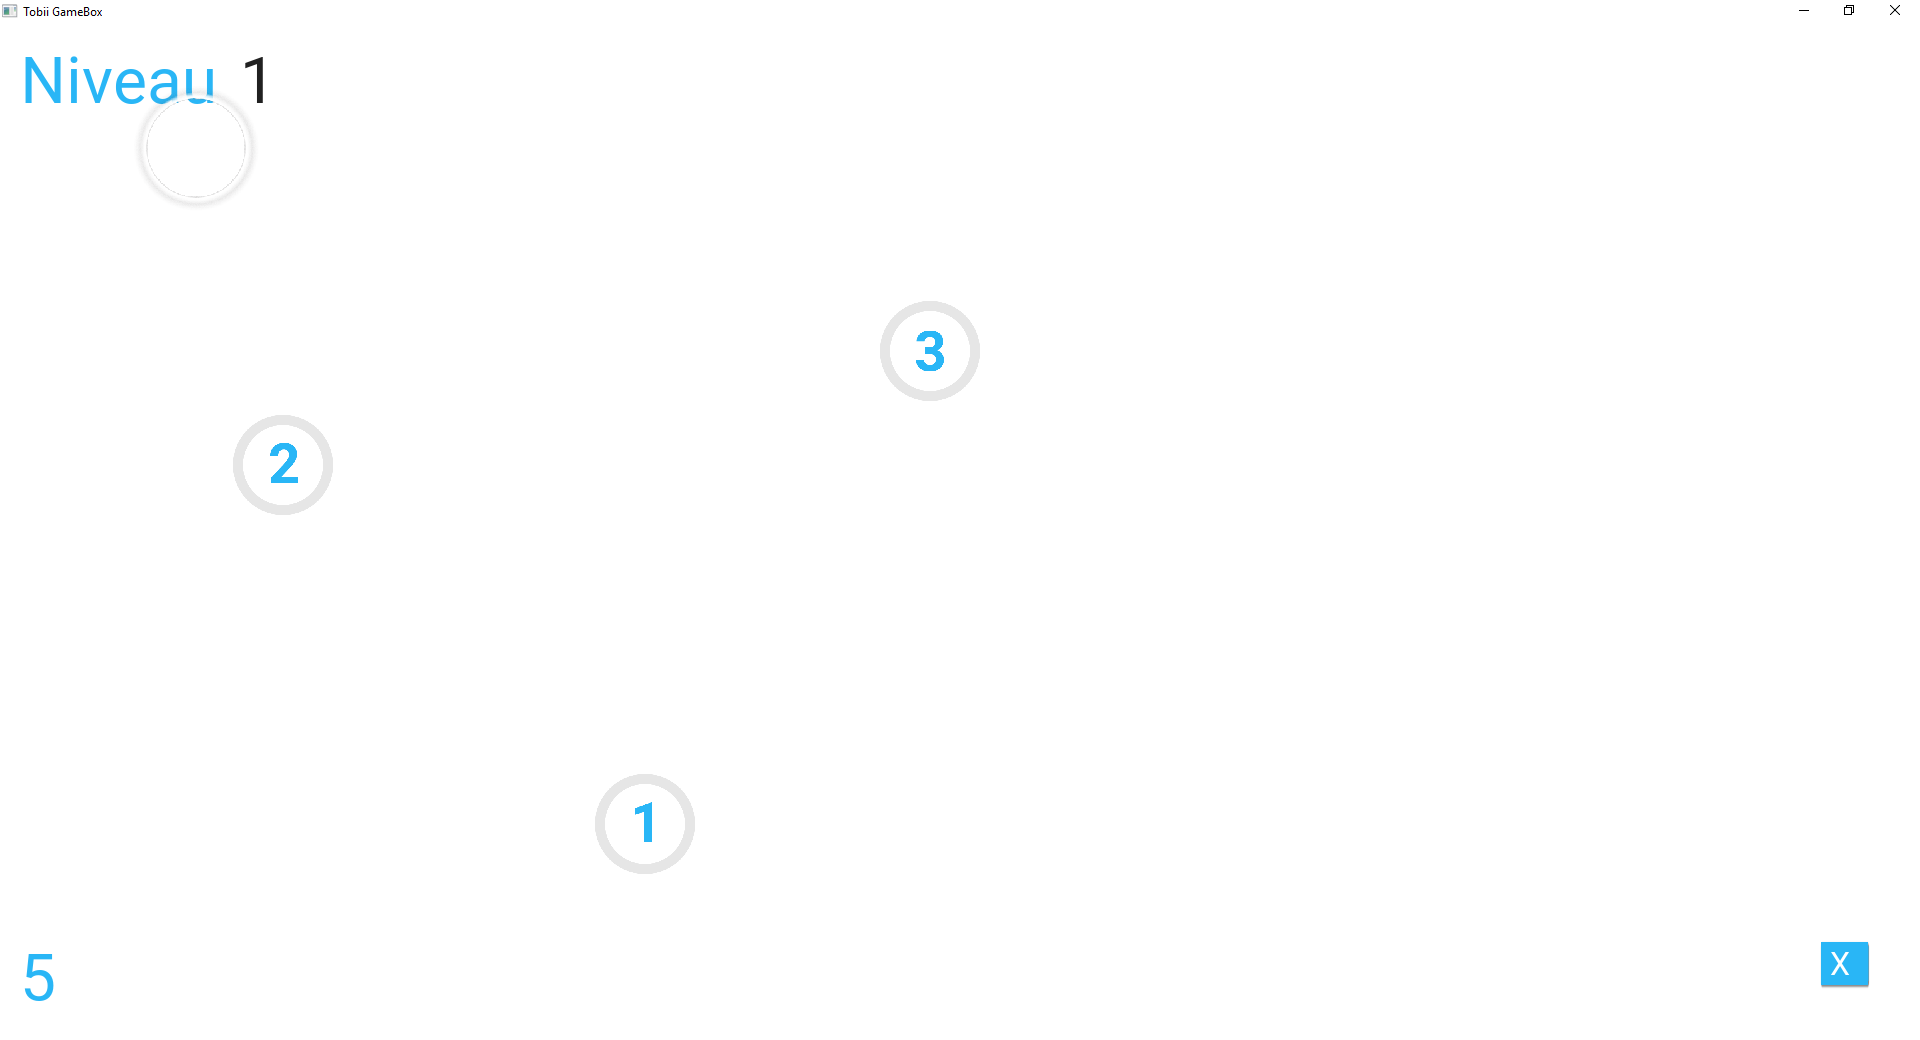
\includegraphics[width=15cm]{img/screenshots/jeu.PNG}
    \caption{Jeu avec les numéros visible}
    \label{fig:screenshot_game}
\end{figure}

\begin{figure}
    \centering
    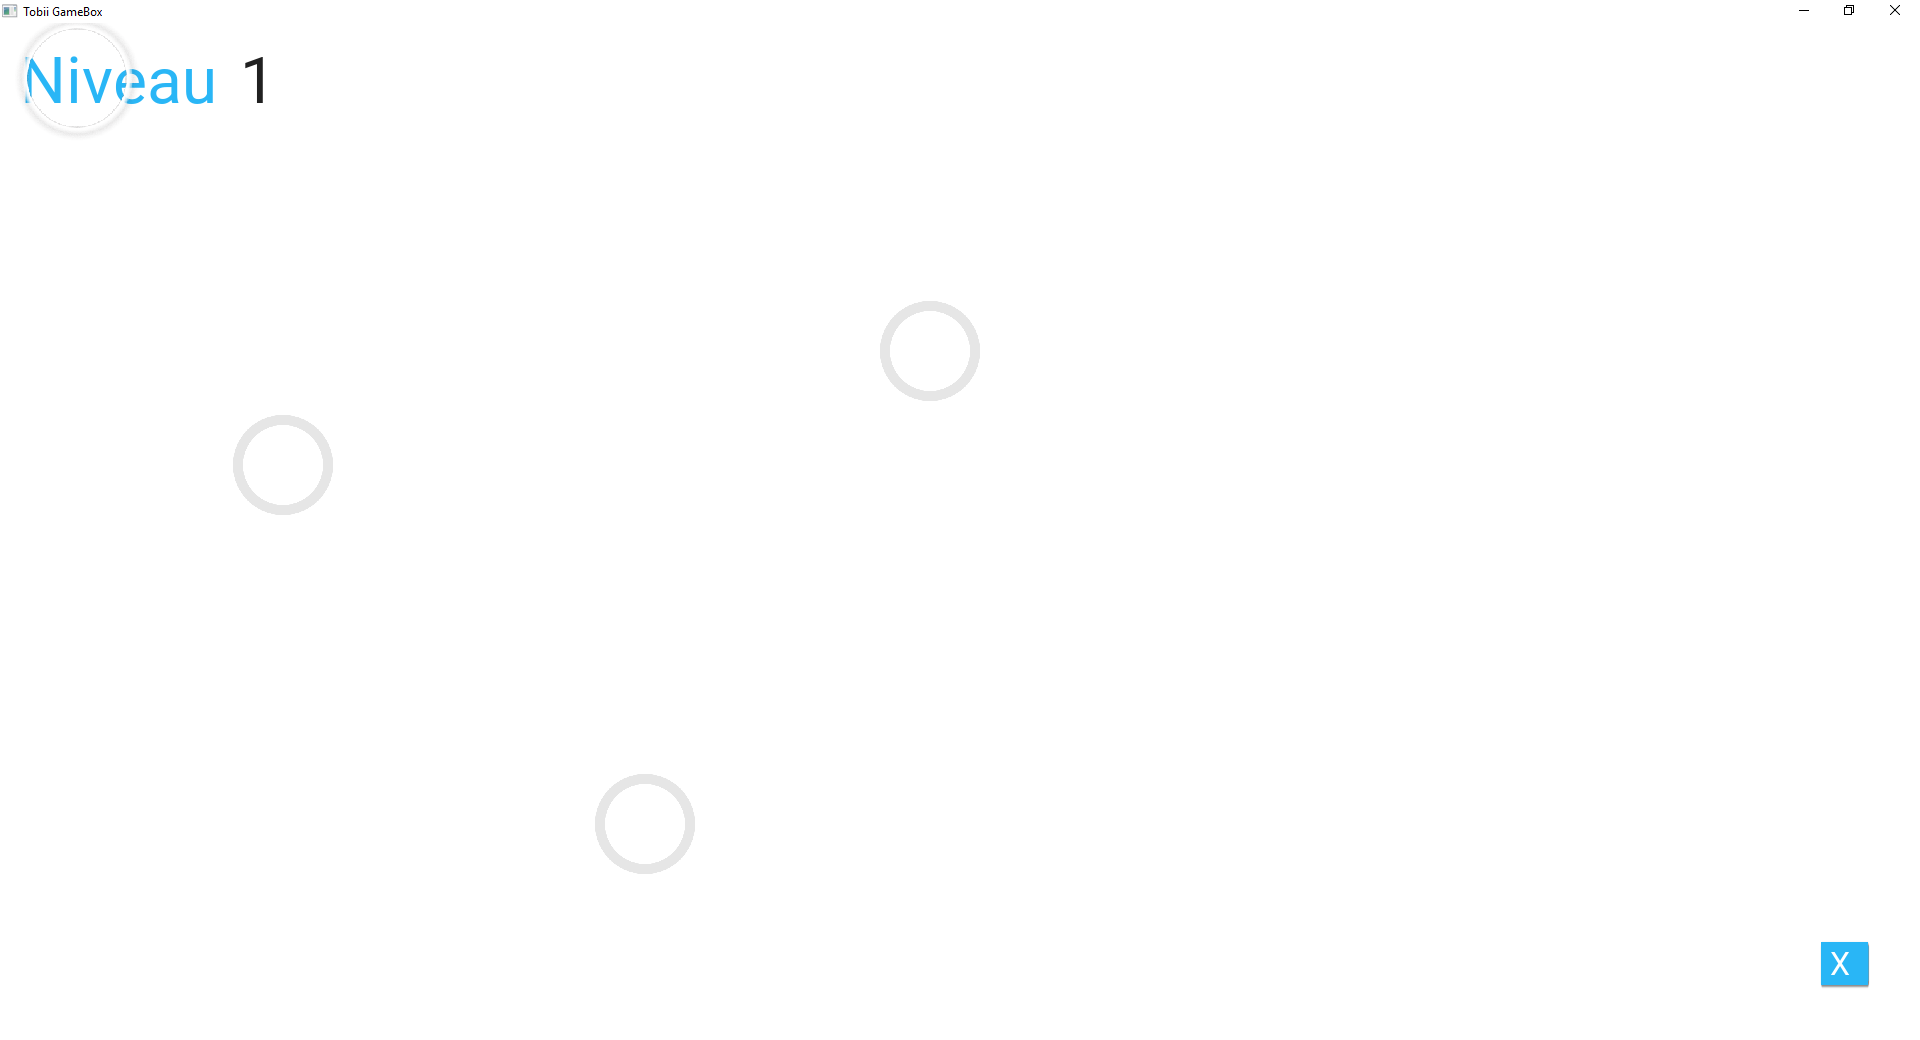
\includegraphics[width=15cm]{img/screenshots/jeu_cachee.PNG}
    \caption{Jeu avec les numéros invisible}
    \label{fig:screenshot_game_invisible}
\end{figure}

\begin{figure}
    \centering
    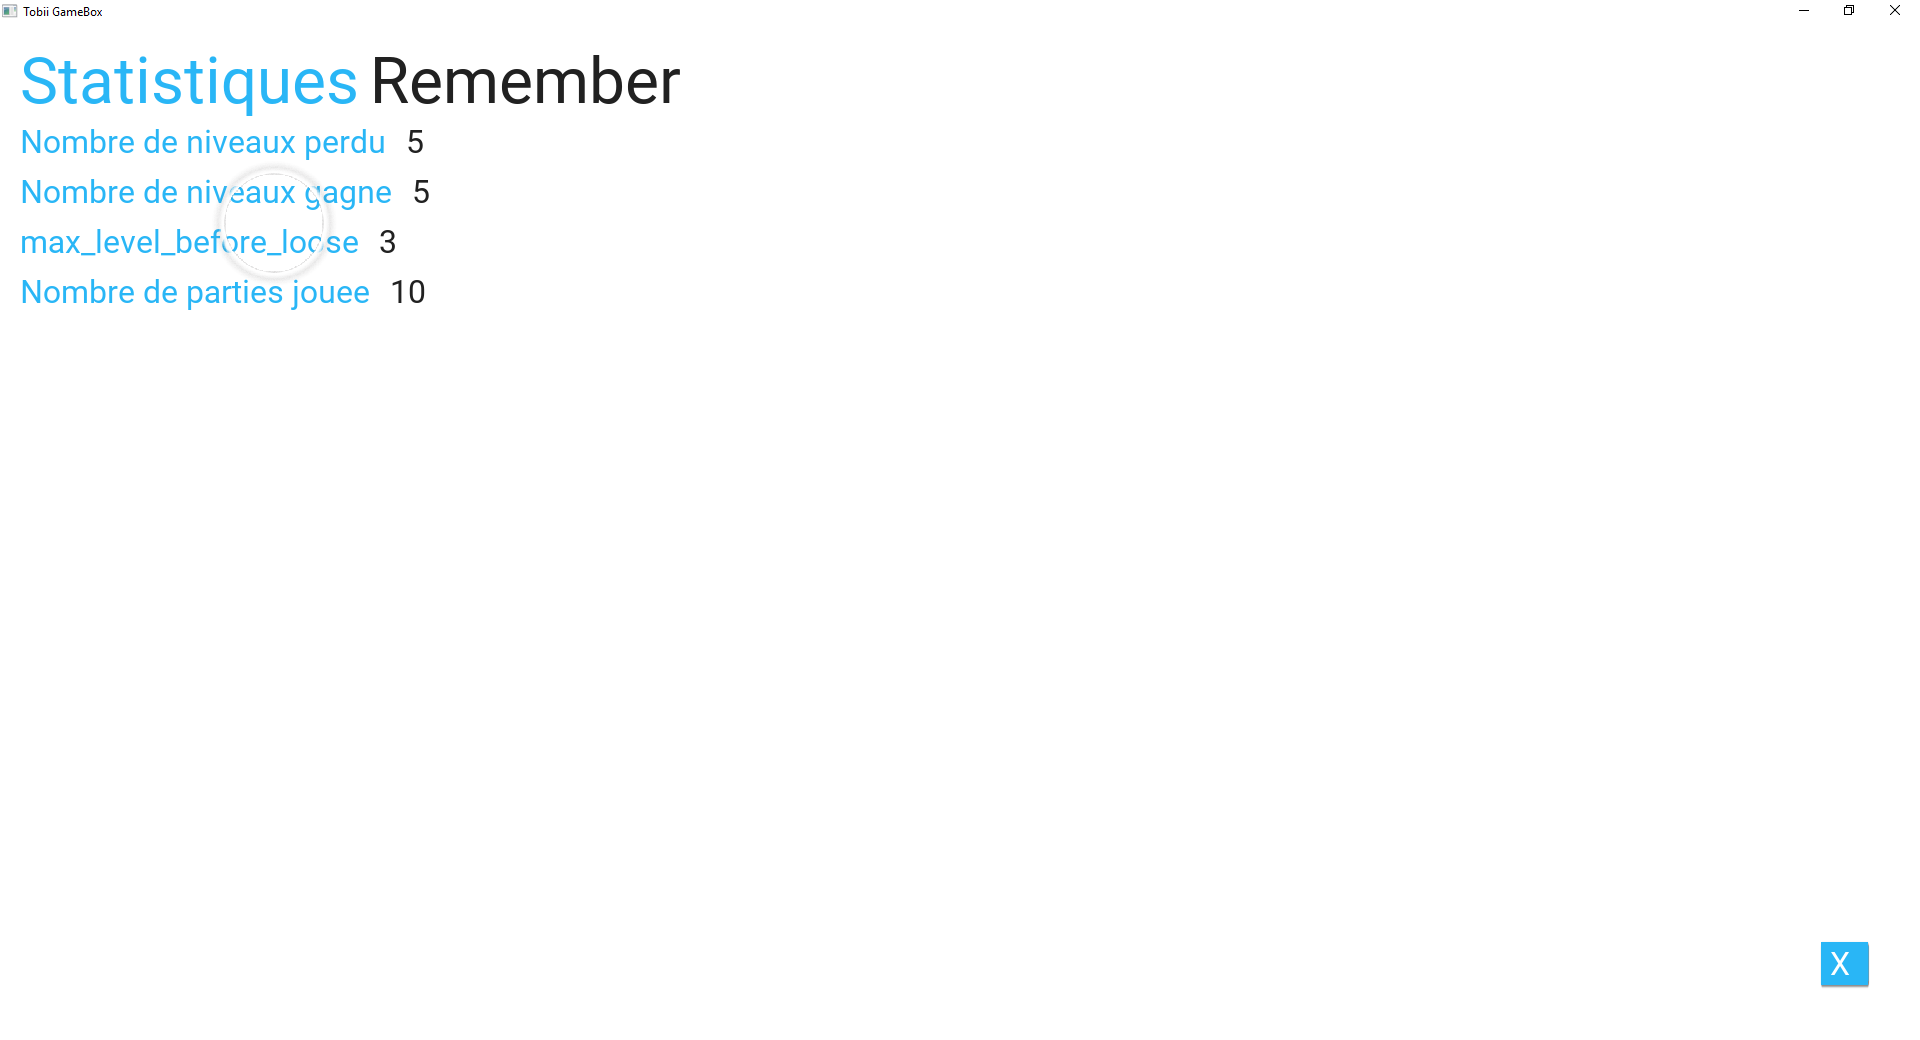
\includegraphics[width=15cm]{img/screenshots/statistiques.PNG}
    \caption{Écran des statistiques}
    \label{fig:screenshot_statistics}
\end{figure}

\chapter*{Conclusion}
Ce projet n'a pas été une totale réussite mais nous avons essayé d'aller le plus loin possible dans la partie développement. Le code réalisé est le plus possible réutilisable et maintenable. Nous avons également produit plusieurs documents de génie logiciel au cours du déroulement du projet dont différents diagrammes UML, une synthèse du cahier des charges et des  spécifications du projet dans la Cahier de spécifications. Nous avons ensuite produit des documents pour le rendu tel qu'un cahier de maintenance et un guide d'utilisation. Tous ces documents et diagrammes nous ont aidé à mieux structurer notre projet pour produire un code de meilleur qualité. 

\weeklyreport{30/09/2018}{Bonjour,

Nous avons terminé de lire les documents que vous nous avez envoyé et nous avons trouvé les projets précédent plutôt intéressant, les documents portant sur le dispositif Tobii étant d'autant plus informatif pour notre projet (contrôle d'un logiciel avec le dispositif Tobii). Nous avons aussi remarqué que les projets précédent, portant sur le même sujet que nous, étaient principalement orientés sur le jeux vidéo. Malgré cela, c'est une des pistes que nous envisageons sérieusement pour notre propre projet et nous voulions donc avoir votre aval pour poursuivre notre réflexion sur ce sujet.

Nous aimerions aussi connaître les disponibilités de la barre Tobii que vous possédez. Nous sommes au courant que nous allons la partager avec un autre groupe, mais nous aimerions lancer les premiers test au plus vite (installation des différents logiciels, prise en main de la barre) afin de connaître les possibilités qui s'offrent à nous. 

Dans le même temps, nous aimerions prévoir avec vous une réunion de début de projet plus spécifique à notre projet. Cela aura pour but de pour discuter de la direction que celui-ci pourra prendre en partageant avec vous les différentes idées que nous avons.

Si vous avez des questions ou des remarques sur notre compte rendu, n’hésitez pas à nous contacter.}

\weeklyreport{14/10/2018}{Bonjour,
Cette semaine nous avons commencé à tester les différents SDK mis à disposition par Tobii. Nous avons testé le SDK pour Unity et celui pour python. Nous n'avons malheureusement pas pu aller très loin étant donné le temps de disponibilité de la barre.
Nous avons aussi commencé à développer avec le framework Pygames. Ce framework permet de développer des jeux (aspect visuel) avec python.
 
Concernant les idées dont nous vous avions fait part, nous avons créé des mockups pour les mettre à plat et dans le but de vous les présenter plus en détail.
C'est pourquoi nous souhaiterions prendre rendez-vous au plus vite pour vous en parler plus en détail. }

\weeklyreport{21/10/2018}{Voici notre compte rendu de la semaine écoulée. Cette semaine, nous avons rédigé le cahier de spécification en suivant le modèle fourni par M.Ragot.
Nous avons également élaboré des mockups pour les différents jeux et menus du notre programme. 
Nous avons en parallèle commencé à développer des briques de notre logiciel en utilisant la librairie PyGames et le SDK Tobii.
Nous avons rencontré quelques problèmes concernant le SDK Tobii. Nous avons commencé à nous mettre en relation avec l'équipe de Tobii France pour les résoudre.

Concernant le compte rendu de la réunion du vendredi 19 octobre.
Lors de cette réunion, nous avons discuté de notre problème avec le SDK Tobii et en sommes venus à la conclusion que nous allions les contacter pour en savoir plus et pour obtenir une licence.
Nous vous avons aussi montré les différents mockups que nous avions réalisé et vous avez validé les idées que nous avons proposées.}

\weeklyreport{28/10/2018}{Voici notre compte rendu hebdomadaire de la semaine.
Cette semaine a été bien chargée au niveau du travail à fournir dans différentes matières, nous n'avons donc pas eu beaucoup de temps pour travailler sur le projet.
Nous avons néanmoins pris le temps de contacter le service client Tobii pour connaître le tarif du SDK que nous voulions utiliser (vous pouvez retrouver les infos dans le mail précèdent).
Suite à cela, nous avons conclu que nous ne pouvions plus utiliser le langage Python et par conséquent, nous avons effectué des recherches pour savoir quel langage utiliser. Nous avons actuellement le choix entre Unity (C\#) et le C++. Cette dernière option nécessite de faire tout manuellement via des bibliothèques externe comme la SDL ou SFML. 
Nous n'avons pas encore choisi d'option et nous sommes encore en train étudier le problème.
Nous vous fournirons une version du cahier de spécification contenant les modifications de langage et de librairies utilisées. }

\weeklyreport{12/11/2018}{Voici notre compte rendu hebdomadaire pour la semaine passée. Nous sommes un peu en retard à cause de nos emplois du temps chargées.
Cette semaine, nous avons commencé à développer le projet en C++ en utilisant le Tobii Stream SDK. Nous sommes pour le moment au début du projet (en terme de programmation) mais la courbe de progression est haute.
Nous avons mis à jour le cahier de spécifications pour qu'il prenne en compte les nouvelles spécifications du projet. Cette version prend en compte le changement de langage et de plus amples spécifications. Vous le trouverez dans les pièces jointes. Pourriez vous le valider et nous donner vos retour dessus ? Merci d'avance. }

\weeklyreport{21/11/2018}{Après cette longue semaine qui s'est écoulé, nous voulions vous tenir au courant de notre avancement dans le projet. 
Comme précisé dans le précédent mail, nous développons finalement notre projet de GameBox en C++ à l'aide du SDK Tobii Stream Engine (voir le cahier de spécification pour plus de détails). 

Du côté de l'interface utilisateur, nous avons d'ores et déjà une fenêtre d'affichage graphique redimensionnable incluant le suivi de la souris ainsi que le suivi du regard grâce au Tobii. Le gaze indiquant la position du curseur suit en priorité le mouvement des yeux sur l'écran quand le Tobii est détecté, sinon c'est la souris qui est prise en compte. A présent, nous nous focalisons sur l'interface graphique à proprement parlé avec, dans un premier temps, la création du menu principal de la GameBox qui permettra la sélection des différents menus ou jeux.

Du côté de la programmation des fonctionnalités, nous avons implémenté un logger pour une meilleure compréhension du code à l'exécution en mode debug ainsi qu'un fichier de configuration permettant de choisir la résolution de la fenêtre (plein écran, fenêtré...). Nous sommes actuellement en train de programmer la détection des jeux qui seront contenu dans le dossier prévu à cet effet, ce qui nous permettra de commencer à créer notre premier jeu par la suite.
 
Au vue de l'avancement du projet et des problèmes rencontrés, nous prévoyons toujours de créer 3 mini-jeux, mais il est possible que ce nombre soit réduit si nous estimons que la qualité de notre production ne soit pas en accord avec les délais. 

En espérant que cela vous conviendra. Si vous avez des questions ou des remarques à propos de notre avancement et de nos prévisions pour la suite du projet, n'hésitez pas à nous en faire part !}

\weeklyreport{25/11/2018}{Voici le compte rendu de la semaine écoulée. 
Durant cette semaine nous avons continué à travailler sur la partie programmation du projet.
Nous nous somme attelé à la réalisation du menu permettant de choisir entre les différents jeux. 
Nous avons pour cela créé divers classes permettant de gérer les textes affichés à l'écran ainsi que les classes correspondant aux boutons.
Nous avons aussi corrigé plusieurs problèmes d'optimisation en relation avec la barre Tobii (reconnexion en cas de problème, etc...).

La semaine prochaine nous prévoyons de terminer le menu et de commencer à réaliser le premier jeu. 
Nous prévoyons aussi de prendre de l'avance sur le rapport que nous allons vous rendre.}

\weeklyreport{3/12/2018}{La semaine passée nous avons continué à programmer le logiciel en développant principalement le menu avec les différentes fonctionnalités disponibles.
Nous avons également réfléchi à la conception du premier jeu que nous allons développer.
En complément, nous avons importé et pris en main les règles LaTex en vu de commencer le rapport.}

\weeklyreport{10/12/2018}{Tout d'abord, nous n'avions pas encore répondu à votre demande de réunion et donc nous sommes disponibles demain à 12h. Nous espérons que cela vous convienne malgré le retard de réponse, veuillez nous en excuser. Pour cette réunion nous prévoyons de vous proposer des diagrammes permettant de mieux exprimer notre avancement et une rapide présentation du projet actuel.

Concernant le projet, nous avons continué à développer le jeu que nous souhaitons réaliser. Nous avons résolu des problèmes d’ergonomie concernant le redimensionnement de l’application. Le premier jeu est en cours de développement. Cela prend du temps car nous sommes en train de mettre en place des outils pour faciliter l’implémentation des autres jeux.}

\weeklyreport{17/12/2018}{Suite à notre réunion du 11 Décembre 2018, nous avons continué le développement de notre projet en suivant vos conseils qui étaient les suivants :
[Réalisé] Ajout d'une sélection du jeu sur le menu principal
[Réalisé] Ajout d'un bouton "Jouer"
[En cours] Sous-menu "Statistiques" et "Leaderboard" propre à chaque jeu
Du côté de notre premier jeu, nous avons implémenté les premières fonctionnalités visant à afficher les différents cercles numérotés de manière aléatoire sur la fenêtre. 
Au vu de l'avancement, nous serons prêt à vous faire une première démonstration de ce nouveau menu principal ainsi que du jeu lors d'une petite réunion en fin de semaine. Pour cela, nous vous proposons Vendredi au alentour de 10h ou de 13h30, mais n'hésitez pas à nous faire part de vos préférences.}

\printbibliography

\end{document}
